\documentclass[12pt]{report}

\usepackage[margin=1in]{geometry}
\usepackage{titlesec}
\usepackage{graphicx}
\usepackage{hyperref}
\usepackage{amsmath}
\usepackage{listings}
\usepackage{enumitem}
\usepackage{array}
\usepackage{booktabs}

\hypersetup{
    colorlinks=true,
    linkcolor=blue,
    urlcolor=blue
}

\lstset{
    basicstyle=\ttfamily\small,
    breaklines=true,
    breakatwhitespace=true,
    columns=fullflexible,
    frame=single
}

\title{
    \textbf{CPE 431 \\ Final Technical Report} \\
    \vspace{0.5cm}
    \textbf{Custom Instruction Set Architecture Design} \\
    \vspace{1cm}
    \large The University of Alabama in Huntsville
}

\author{Esther Shore \\
Department of Electrical \& Computer Engineering}

\date{December 9, 2025}

\begin{document}

\maketitle
\pagenumbering{roman}
% \begin{abstract}
% \end{abstract}
\tableofcontents
\clearpage
\pagenumbering{arabic}

\chapter{Introduction}

This project presents the design of a custom 16-bit RISC-style instruction set
architecture (ISA) intended for a simple, low-cost microprocessor. The ISA is
restricted to no more than sixteen instructions, each encoded in a single
16-bit word. All operands are 16-bit two's-complement integers, and the
processor operates on a linear, word-addressable memory space consisting of
1024 words.

The ISA follows RISC design principles by using a small register file,
regular instruction formats, and simple addressing modes. A dedicated zero
register and a link register support core programming patterns while keeping
the hardware lightweight.

Despite its small size, the ISA supports all required C programming language
constructs, including arithmetic and logical expressions, assignments,
one-dimensional arrays, relational operators, conditional branches, loops, and
function calls with parameters passed by value or reference. A HALT
instruction is included to terminate program execution.

The following chapters describe the instruction formats, register set,
complete instruction definitions, compilation examples, and the HDL
implementation of the processor.


\chapter{User-Programmable Registers}

The processor contains eight 16-bit general-purpose registers, numbered \texttt{0-7}.
Register \texttt{\$zero} is hardwired to the constant value 0. Registers \texttt{\$r1}
through \texttt{\$r6} are programmer-visible general-purpose registers used for
arithmetic, addressing, and temporary storage. Register \texttt{\$ra} is used
as the link register during function calls.

\begin{table}[h!]
\centering
\begin{tabular}{|c|c|l|}
\hline
\textbf{Name} & \textbf{Number} & \textbf{Description} \\ \hline
\texttt{\$zero} & 0 & Constant value 0 \\ \hline
\texttt{\$r1-\$r6} & 1--6 & General-purpose registers for computation and addressing \\ \hline
\texttt{\$ra} & 7 & Return address register for function calls \\ \hline
\end{tabular}
\caption{Register File Summary}
\end{table}


\chapter{Instruction Formats}

This architecture supports three instruction formats: Register-type (R), Load/Store-type (LS), and Immediate/Jump-type (IJ).  
Each instruction is encoded into a 16-bit word in a word-addressable 1~KiB memory space.

\section{Register Format (R)}
\[
\text{op}_{15:13} \;\vert\; \text{rs}_{12:10} \;\vert\; \text{rt/imm3}_{9:7} \;\vert\; 
\text{rd}_{6:4} \;\vert\; \text{funct}_{3:1} \;\vert\; \text{iflag}_{0}
\]
This format allows two register operands and one destination register.  
A single-bit immediate flag distinguishes pure register operations from short-immediate encoded ALU operations.

\section{Load/Store Format (LS)}
\[
\text{op}_{15:13} \;\vert\; \text{rs}_{12:10} \;\vert\; \text{rt}_{9:7} \;\vert\; 
\text{imm7}_{6:0}
\]
This supports base+offset addressing for memory operands.

\section{Immediate/Jump Format (IJ)}
\[
\text{op}_{15:13} \;\vert\; \text{rd}_{12:10} \;\vert\; 
\text{imm10}_{9:0}
\]
Used for large immediates, conditional branches, and jump instructions.

\clearpage

\chapter{Instruction Set Architecture}

\section{Instruction Summary}

Table~\ref{tab:isa-summary} provides an overview of all sixteen instructions
in the ISA, including opcode/funct fields, instruction type, and a brief 
description of behavior.

\begin{table}[h!]
\centering
\small
\begin{tabular}{cccc}
\toprule
\textbf{Op/Funct} & \textbf{Mnemonic} & \textbf{Type} & \textbf{Description} \\
\midrule
000 / 111 & HALT & R & Stop execution \\ 
000 / 000 & ADD  & R & $R[rd] \leftarrow R[rs] + R[rt]$ \\ 
000 / 001 & SUB  & R & $R[rd] \leftarrow R[rs] - R[rt]$ \\ 
000 / 010 & AND  & R & $R[rd] \leftarrow R[rs] \;\&\; R[rt]$ \\ 
000 / 011 & OR   & R & $R[rd] \leftarrow R[rs] \;|\; R[rt]$ \\ 
000 / 100 & SLT  & R & $R[rd] \leftarrow (R[rs] < R[rt]) ? 1 : 0$ \\ 
000 / 101\textsuperscript{*} & SLL  & R & $R[rd] \leftarrow R[rs] \ll \text{signext(imm3)}$ \\ 
000 / 110\textsuperscript{*} & SRL  & R & $R[rd] \leftarrow R[rs] \gg \text{signext(imm3)}$ \\ 
000 / 000\textsuperscript{*} & ADDI & R & $R[rd] \leftarrow R[rs] + \text{signext(imm3)}$ \\ 
\midrule
001 & ST  & LS & $M[R[rs] + \text{signext(imm7)}] \leftarrow R[rt]$ \\ 
010 & LD  & LS & $R[rt] \leftarrow M[R[rs] + \text{signext(imm7)}]$ \\ 
\midrule
011 & LDI & IJ & $R[rd] \leftarrow \text{signext(imm10)}$ \\ 
100 & BEZ & IJ & If $R[rd] = 0$: $PC \leftarrow PC + 1 + \text{signext(imm10)}$ \\ 
101 & BNZ & IJ & If $R[rd] \neq 0$: $PC \leftarrow PC + 1 + \text{signext(imm10)}$ \\ 
110 & JL  & IJ & $R[ra] \leftarrow PC + 1$, $PC \leftarrow \text{imm10}$ \\ 
111 & JR  & IJ & $PC \leftarrow R[rs]$ \\ 
\bottomrule
\end{tabular}
\caption{Summary of ISA Instructions}
\label{tab:isa-summary}
\end{table}

\noindent\textbf{*} Instructions SLL, SRL, and ADDI use the R-type format with \textit{iflag = 1},  
indicating that bits [9:7] represent a 3-bit immediate instead of register \texttt{rt}.

\section{Arithmetic Instructions}

\subsection*{ADD}
\textbf{Assembly:} \texttt{ADD rd, rs, rt} \\
\textbf{Encoding:} op=000, funct=000, iflag=0 
\[
000 \;|\; rs \;|\; rt \;|\; rd \;|\; 000 \;|\; 0
\]
\textbf{Operation:} \( R[rd] \leftarrow R[rs] + R[rt] \) \\
\textbf{Justification:} Core integer arithmetic operation.

\vspace{1em}

\subsection*{SUB}

\textbf{Assembly:} \texttt{SUB rd, rs, rt} \\
\textbf{Encoding:} op=000, funct=001, iflag=0 
\[
000 \;|\; rs \;|\; rt \;|\; rd \;|\; 001 \;|\; 0
\]
\textbf{Operation:} \( R[rd] \leftarrow R[rs] - R[rt] \) \\
\textbf{Justification:} Required for comparisons, indexing, and loop control.

\vspace{1em}

\subsection*{ADDI}
\textbf{Assembly:} \texttt{ADDI rd, rs, imm3} \\
\textbf{Encoding:} op=000, funct=000, iflag=1 
\[
000 \;|\; rs \;|\; imm3 \;|\; rd \;|\; 000 \;|\; 1
\]
\textbf{Operation:} \( R[rd] \leftarrow R[rs] + \text{signext(imm3)} \) \\
\textbf{Justification:} Efficient small constant arithmetic for increments, stack offsets, and loop updates.

\section{Logical Instructions}

\subsection*{AND}
\textbf{Assembly:} \texttt{AND rd, rs, rt} \\
\textbf{Encoding:} op=000, funct=010, iflag=0 
\[
000 \;|\; rs \;|\; rt \;|\; rd \;|\; 010 \;|\; 0
\]
\textbf{Operation:} \( R[rd] \leftarrow R[rs] \;\&\; R[rt] \) (bitwise AND)\\
\textbf{Justification:} Logical masking and bit operations.

\vspace{1em}

\subsection*{OR}
\textbf{Assembly:} \texttt{OR rd, rs, rt} \\
\textbf{Encoding:} op=000, funct=011, iflag=0 
\[
000 \;|\; rs \;|\; rt \;|\; rd \;|\; 011 \;|\; 0
\]
\textbf{Operation:} \( R[rd] \leftarrow R[rs] \;|\; R[rt] \) (bitwise OR)\\
\textbf{Justification:} Setting or combining bitfields.

\vspace{1em}

\subsection*{SLT}
\textbf{Assembly:} \texttt{SLT rd, rs, rt} \\
\textbf{Encoding:} op=000, funct=100, iflag=0 
\[
000 \;|\; rs \;|\; rt \;|\; rd \;|\; 100 \;|\; 0
\]
\textbf{Operation:} \( R[rd] \leftarrow 1 \text{ if } (R[rs] < R[rt]) \text{ else } 0 \) (signed) \\
\textbf{Justification:} Enables full C-level relational comparisons.

\vspace{1em}

\subsection*{SLL}
\textbf{Assembly:} \texttt{SLL rd, rs, imm3} \\
\textbf{Encoding:} op=000, funct=101, iflag=1 
\[
000 \;|\; rs \;|\; imm3 \;|\; rd \;|\; 101 \;|\; 1
\]
\textbf{Operation:} \( R[rd] \leftarrow R[rs] \ll \text{imm3} \) (logic shift left) \\
\textbf{Justification:} Efficient shifts for multiplication and bit-field construction.

\vspace{1em}

\subsection*{SRL}
\textbf{Assembly:} \texttt{SRL rd, rs, imm3} \\
\textbf{Encoding:} op=000, funct=110, iflag=1 
\[
000 \;|\; rs \;|\; imm3 \;|\; rd \;|\; 110 \;|\; 1
\]
\textbf{Operation:} \( R[rd] \leftarrow R[rs] \gg \text{imm3} \) (logical shift right) \\
\textbf{Justification:} Logical right shifts for bit extraction and unsigned division by powers of two.

\section{Memory Instructions}

\subsection*{LD}
\textbf{Assembly:} \texttt{LD rt, imm7(rs)} \\
\textbf{Encoding:} op=010 
\[
010 \;|\; rs \;|\; rt \;|\; imm7
\]
\textbf{Operation:} \( R[rt] \leftarrow M[R[rs] + \text{signext(imm7)}] \) \\
\textbf{Justification:} Loads stack variables, arrays, and memory operands.

\vspace{1em}

\subsection*{ST}
\textbf{Assembly:} \texttt{ST rt, imm7(rs)} \\
\textbf{Encoding:} op=001 
\[
001 \;|\; rs \;|\; rt \;|\; imm7
\]
\textbf{Operation:} \( M[R[rs] + \text{signext(imm7)}] \leftarrow R[rt] \) \\
\textbf{Justification:} Required for storing variables and function call frames.

\vspace{1em}

\subsection*{LDI}
\textbf{Assembly:} \texttt{LDI rd, imm10} \\
\textbf{Encoding:} op=011 
\[
011 \;|\; rd \;|\; imm10
\]
\textbf{Operation:} \( R[rd] \leftarrow \text{signext(imm10)} \) \\
\textbf{Justification:} Loads large constants and full 10-bit addresses.

\section{Control Flow Instructions}

\subsection*{BEZ}
\textbf{Assembly:} \texttt{BEZ rd, offset} \\
\textbf{Encoding:} op=100 
\[
100 \;|\; rd \;|\; imm10
\]
\textbf{Operation:} If \( R[rd] = 0 \), then  
\[
PC \leftarrow PC + 1 + \text{signext(imm10)}
\]
\textbf{Justification:} Implements if-statements, while-loops, and loop exits.

\vspace{1em}

\subsection*{BNZ}
\textbf{Assembly:} \texttt{BNZ rd, offset} \\
\textbf{Encoding:} op=101 
\[
101 \;|\; rd \;|\; imm10
\]
\textbf{Operation:} If \( R[rd] \neq 0 \), branch relative. \\
\textbf{Justification:} Complements BEZ for full branch support.

\vspace{1em}

\subsection*{JL}
\textbf{Assembly:} \texttt{JL imm10} \\
\textbf{Encoding:} op=110, rd fixed to \$ra 
\[
110 \;|\; 111 \;|\; imm10
\]
\textbf{Operation:}  
\[
R[ra] \leftarrow PC + 1, \qquad PC \leftarrow imm10
\]
\textbf{Justification:} Enables direct function calls with automatic return address storage.

\vspace{1em}

\subsection*{JR}
\textbf{Assembly:} \texttt{JR rs} \\
\textbf{Encoding:} op=111 
\[
111 \;|\; rs \;|\; 0000000000
\]
\textbf{Operation:} \( PC \leftarrow R[rs] \) \\
\textbf{Justification:} Function return and indirect jump.

\section{HALT Instruction}

\subsection*{HALT}
\textbf{Assembly:} \texttt{HALT} \\
\textbf{Encoding:} op=000, funct=000, iflag=0 
\[
000 \;|\; 000 \;|\; 000 \;|\; 000 \;|\; 111 \;|\; 0
\]
\textbf{Operation:} Stop execution. \\
\textbf{Justification:} Allows simulator and hardware to terminate safely.

\section{Constructing Full 16-Bit Immediates}

Because the ISA supports only a 10-bit immediate field in the \texttt{LDI}
instruction, a full 16-bit constant cannot be encoded in a single instruction.
However, any 16-bit value can be constructed using a standard sequence consisting
of loading the upper byte, shifting it into position, and merging in the lower
byte.

\subsection*{Method Overview}

\begin{enumerate}
    \item Use \texttt{LDI} to load the upper 8 bits of the constant into a
          register.
    \item Shift the value left by 8 positions using three \texttt{SLL}
          instructions (since only 3-bit signed shift amounts are supported):
          \( 3 + 3 + 2 = 8 \).
    \item Use a second \texttt{LDI} to load the lower 8 bits.
    \item Combine the high and low bytes using the \texttt{OR} instruction.
\end{enumerate}

This procedure allows construction of any 16-bit constant.

\subsection*{Example: Loading the Constant \texttt{0xABCD}}

We wish to place the 16-bit value \texttt{0xABCD} into \texttt{r1}.

\begin{lstlisting}
    LDI  r1, 0xAB      ; load upper byte
    SLL  r1, r1, 3     ; shift left by 3: << 3
    SLL  r1, r1, 3     ; shift left by 3: << 6
    SLL  r1, r1, 2     ; shift left by 2: << 8 total (now r1 = 0xAB00)

    LDI  r2, 0xCD      ; load lower byte
    OR   r1, r1, r2    ; combine halves --> r1 = 0xABCD
\end{lstlisting}

\subsection*{Result}

After executing the sequence, the register contains the full 16-bit constant:
\[
    r1 = 0xABCD.
\]

This approach works for all 16-bit values and relies solely on instructions
already present in the ISA (\texttt{LDI}, \texttt{SLL}, and \texttt{OR}), without
modifying the instruction formats or adding new opcodes.

\clearpage

\chapter{Compiling C Constructs}

This chapter demonstrates how each required C-language programming construct is translated into the custom ISA.

\section{If--Else}

\subsection*{C Code}
\begin{lstlisting}
if (a < b) {
    x = y;
} else {
    x = z;
}
\end{lstlisting}

\subsection*{Assembly}
\begin{lstlisting}
    ; Assume:
    ;   a in R1, b in R2
    ;   x in R3, y in R4, z in R5
    ;   R6 is temporary
    SLT  R6, R1, R2        ; R6 = (a < b)
    BEZ  R6, else          ; if condition is false, jump to else-block
    ADD  R3, R4, R0        ; then-block: x = y
    BNZ  R6, endif         ; skip else-block
else:
    ADD  R3, R5, R0        ; else-block: x = z
endif:
\end{lstlisting}

\section{While Loop}

\subsection*{C Code}
\begin{lstlisting}
while (i < n) {
    i = i + 1;
}
\end{lstlisting}

\subsection*{Assembly}
\begin{lstlisting}
    ; Assume:
    ;   i in R1, n in R2
    ;   R3 is temporary
loop:
    SLT  R3, R1, R2        ; R3 = (i < n)
    BEZ  R3, end           ; exit loop when condition is false
    ADDI R1, R1, 1         ; i = i + 1
    BNZ  R3, loop          ; repeat loop while previous condition was true
end:
\end{lstlisting}

\section{For Loop}

\subsection*{C Code}
\begin{lstlisting}
for (i = 0; i < n; i++) {
    sum += i;
}
\end{lstlisting}

\subsection*{Assembly}
\begin{lstlisting}
    ; Assume:
    ;   i   in R1
    ;   n   in R2
    ;   sum in R3
    ;   R4 is temporary
    LDI  R1, 0             ; i = 0
for_loop:
    SLT  R4, R1, R2        ; R4 = (i < n)
    BEZ  R4, done          ; exit loop when i >= n
    ADD  R3, R3, R1        ; sum += i
    ADDI R1, R1, 1         ; i++
    BNZ  R4, for_loop      ; repeat loop while condition was true
done:
\end{lstlisting}

\section{Relational Operators}

In all examples below, we assume:
\begin{itemize}
    \item \texttt{a} is stored in register \texttt{r1}
    \item \texttt{b} is stored in register \texttt{r2}
    \item \texttt{r3} is a temporary register used for comparisons
    \item Labels such as \texttt{IF\_TRUE} are resolved to appropriate PC-relative offsets by the assembler.
\end{itemize}

Each relational operator is implemented as a minimal \texttt{if} statement without an \texttt{else} block to show that the ISA can drive a conditional branch.

\subsection*{Equality: \texorpdfstring{$==$}{==}}

\begin{lstlisting}
// C: if (a == b) { /* then */ }

SUB  r3, r1, r2      ; r3 = a - b
BEZ  r3, IF_TRUE     ; if (a == b) branch
\end{lstlisting}

\subsection*{Not Equal: \texorpdfstring{$!=$}{!=}}

\begin{lstlisting}
// C: if (a != b) { /* then */ }

SUB  r3, r1, r2      ; r3 = a - b
BNZ  r3, IF_TRUE     ; if (a != b) branch
\end{lstlisting}

\subsection*{Less Than: \texorpdfstring{$<$}{<}}

\begin{lstlisting}
// C: if (a < b) { /* then */ }

SLT  r3, r1, r2      ; r3 = (a < b) ? 1 : 0
BNZ  r3, IF_TRUE     ; if (a < b) branch
\end{lstlisting}

\subsection*{Less Than or Equal: \texorpdfstring{$<=$}{<=}}

Using the identity $a \le b \Leftrightarrow \neg (a > b) \Leftrightarrow \neg (b < a)$:

\begin{lstlisting}
// C: if (a <= b) { /* then */ }

SLT  r3, r2, r1      ; r3 = (b < a) ? 1 : 0   // a > b
BEZ  r3, IF_TRUE     ; if !(a > b) -> (a <= b) branch
\end{lstlisting}

\subsection*{Greater Than: \texorpdfstring{$>$}{>}}

Using the identity $a > b \Leftrightarrow b < a$:

\begin{lstlisting}
// C: if (a > b) { /* then */ }

SLT  r3, r2, r1      ; r3 = (b < a) ? 1 : 0
BNZ  r3, IF_TRUE     ; if (a > b) branch
\end{lstlisting}

\subsection*{Greater Than or Equal: \texorpdfstring{$>=$}{>=}}

Using the identity $a \ge b \Leftrightarrow \neg (a < b)$:

\begin{lstlisting}
// C: if (a >= b) { /* then */ }

SLT  r3, r1, r2      ; r3 = (a < b) ? 1 : 0
BEZ  r3, IF_TRUE     ; if !(a < b) -> (a >= b) branch
\end{lstlisting}

\noindent
These minimal patterns demonstrate that each C relational operator can be mapped to a short sequence using only \texttt{SUB}, \texttt{SLT}, \texttt{BEZ}, and \texttt{BNZ}.

\section{Function Call and Return}

\subsection{Pass by Value}

This example shows a simple function that increments a value by one and returns it. The argument is passed in \texttt{r1}, and the return value is also placed in \texttt{r1}. Register \texttt{r7} is used as the link register (\texttt{\$ra}) by the \texttt{JL} and \texttt{JR} instructions.

\subsubsection*{C Code}

\begin{lstlisting}
int inc_val(int x) {
    return x + 1;
}

void main(void) {
    int y;
    y = inc_val(10);
}
\end{lstlisting}

\subsubsection*{Assembly Implementation}

\textbf{Caller (main):}
\begin{lstlisting}
    LDI  r1, 10         ; x = 10 (argument in r1)
    JL   INC_VAL        ; jump to function, save return address in r7
    ; on return, r1 holds x + 1 = 11
    ; y can be stored from r1 if needed
\end{lstlisting}

\noindent \textbf{Callee (function \texttt{inc\_val}):}
\begin{lstlisting}
INC_VAL:
    ADDI r1, r1, 1      ; r1 = r1 + 1
    JR   r7             ; return to caller
\end{lstlisting}

This demonstrates call-by-value: the function operates on a copy of the argument in \texttt{r1} and returns the new value in the same register.


\subsection{Pass by Reference}

To demonstrate call-by-reference, a pointer to a variable in memory is passed to the function. The function dereferences the pointer, modifies the value in memory, and returns.

Assume a unified memory where \texttt{x} is stored at address \texttt{X\_ADDR}. Register \texttt{r2} holds the address of \texttt{x}.

\subsubsection*{C Code}

\begin{lstlisting}
void inc_ref(int *p) {
    (*p) = (*p) + 1;
}

void main(void) {
    int x = 7;
    inc_ref(&x);
}
\end{lstlisting}

\subsubsection*{Assembly Implementation}

\textbf{Caller (main):}
\begin{lstlisting}
    LDI  r1, 7              ; x = 7
    LDI  r2, X_ADDR         ; r2 = &x
    ST   r1, 0(r2)          ; M[X_ADDR] = 7

    JL   INC_REF            ; call inc_ref(&x)

    LD   r3, 0(r2)          ; r3 = x, should now be 8
\end{lstlisting}

\noindent \textbf{Callee (function \texttt{inc\_ref}):}
\begin{lstlisting}
INC_REF:
    LD   r4, 0(r2)          ; r4 = *p
    ADDI r4, r4, 1          ; r4 = r4 + 1
    ST   r4, 0(r2)          ; *p = r4
    JR   r7                 ; return to caller
\end{lstlisting}

In this example, the function receives the address of \texttt{x} in \texttt{r2}, operates directly on memory via \texttt{LD} and \texttt{ST}, and therefore implements true call-by-reference semantics.



\chapter{Design Implementation}
\section{Overall Design}

The processor implements the proposed 16-bit RISC ISA using a single-cycle
datapath in which every instruction completes in one clock cycle. The design
includes:

\begin{itemize}
    \item \textbf{PC and Next-PC Logic:} word-addressed program counter with
          sequential (\texttt{PC+1}), branch, and jump paths.
    \item \textbf{Register File:} 8×16 registers with \texttt{r0} hard-wired to
          zero and \texttt{r7} used as the link register.
    \item \textbf{Unified Memory:} a 1\,KiB word-addressable memory shared by
          instructions and data, simplifying initialization and address
          calculations.
    \item \textbf{ALU:} supports ADD, SUB, AND, OR, SLT, SLL, and SRL, plus a
          zero flag for branches.
    \item \textbf{Sign-Extension Units:} handle 3-, 7-, and 10-bit immediates
          for R-, LS-, and IJ-type formats.
    \item \textbf{Control Unit:} decodes \texttt{opcode} and \texttt{funct} and
          directly generates all datapath control signals, including branch and
          jump control and HALT.
\end{itemize}

These components directly support the three ISA formats (R, LS, IJ) and enable
arithmetic, memory access, branches, and function calls/returns exactly as
specified.

\section{Design Changes}

Several refinements were made between the progress report and final
implementation:

\begin{itemize}
    \item \textbf{Unified Control:} merged the main control and ALU-control
          units into one module, simplifying decode and HALT behavior.
    \item \textbf{Unified Memory:} replaced separate instruction/data memories
          with a single module matching the ISA’s flat address space and making
          testbench initialization easier.
    \item \textbf{Improved Immediate Handling:} clean sign-extension logic for
          all immediate sizes and correct selection paths for ADDI, LS-type
          offsets, and IJ-type branches/jumps.
    \item \textbf{Stable HALT Semantics:} HALT cleanly disables PC updates and
          all write enables, freezing the machine state and acting distinctly from a NOP.
\end{itemize}

Overall, the final design is a streamlined and fully verified single-cycle
implementation of the proposed ISA, with simplified control logic, a unified
memory structure, and complete support for conditionals, loops, and
function calls.

\section{Future Improvements}

Several enhancements could extend the capability, robustness, and clarity of
the current single-cycle design:

\begin{itemize}
    \item \textbf{Pipelining:} Introducing a basic multi-stage pipeline would
        improve throughput and increase achievable clock frequency, at the
        cost of hazard detection and forwarding logic.
    \item \textbf{Instruction Formats and Immediate Handling:} Enlarging immediate fields or
        adding more robust instruction formats, utilizing zero-extension
        paths alongside sign-extension would make the datapath cleaner and
        more flexible for future ISA extensions.
    \item \textbf{Simplified MUX Structure:} Consolidating scattered control
        muxes into a smaller number of parameterized multiplexers
        would reduce control complexity and improve readability.
    \item \textbf{More Thorough Unit Tests:} Expanding unit tests for the ALU,
        register file, memory, sign-extension, and control unit—along with
        randomized and corner-case testing—would further increase confidence
        in correctness beyond the directed programs used here.
    \item \textbf{Exception/Interrupt Support:} A minimal exception model would
        enable system calls, timers, and more robust program execution.
\end{itemize}

These improvements provide clear next steps for evolving the processor beyond
the baseline single-cycle ISA implementation and strengthening its verification.


\chapter{Testbench Simulation Output}
\section{Individual Instructions}
Overall, the \texttt{tb\_cpu} testbench verifies the correctness of the core
datapath, control logic, and instruction semantics by executing all sixteen instructions in the ISA. Because
this design implements a single-cycle architecture, each instruction fully
executes in one clock cycle, and the testbench output reflects this.

The complete console output is included below. Each block corresponds to one
clock cycle edge and reports:

\begin{itemize}
    \item The current simulation time and program counter (PC).
    \item The fetched instruction and its decoded fields (opcode, registers,
          funct, and \texttt{iflag}).
    \item The intended meaning of the instruction (\texttt{INST}/\texttt{RTL}).
    \item Control-unit outputs such as register write, memory access, branch and
          jump signals, and the halt flag.
    \item ALU inputs and output, including the zero flag.
    \item Write-back destination and data value.
    \item A snapshot of all architectural registers.
    \item A small window of memory used during execution.
\end{itemize}

To interpret the log, the reader may follow the PC through the program and
confirm that:

\begin{enumerate}
    \item Each instruction is fetched, decoded, executed, and written back
          within a single clock cycle.
    \item ALU operations produce correct arithmetic and logical results.
    \item Register and memory updates match the ISA specification.
    \item Branches and jumps modify the PC precisely as defined.
    \item The processor enters and remains in the halted state after executing
          \texttt{HALT}.
\end{enumerate}

The final register and memory dump at the end of the transcript matches the
expected architectural state:

\begin{itemize}
    \item ALU-based R-type instructions produce correct results in
          \texttt{r3}--\texttt{r6},
    \item \texttt{SLT} correctly sets comparison outcomes,
    \item \texttt{ST}/\texttt{LD} correctly store and retrieve the value 13 at
          memory address~31, and
    \item \texttt{JL}/\texttt{JR} correctly implement a function call and return
          by managing the link register \texttt{r7}.
\end{itemize}

The full cycle-by-cycle console trace of program execution is reproduced below
for reference.

\subsection*{cpu\_tb.v output trace}
\begin{lstlisting}
# Loading work.tb_cpu(fast)
run -all
# ----- t=0 (RESET ACTIVE) -----
# PC = x
# -----------------------------
# 
# ----- t=10 (RESET ACTIVE) -----
# PC = 0
# -----------------------------
# 
# ----- t=20 -----
# PC     = 0
# INSTR  = 0x640a
# DECODE : opcode=011 rs=1 rt=0 rd=0 funct=101 iflag=0
# INST   : [PC 0] LDI r1, 10
# RTL    : r1 = 10
# CONTROL: alu_op=000 reg_dst=010 reg_write=1 mem_read=0 mem_write=1 branch_ez=0 branch_nz=0 imm_jump=0 reg_jump=0 return_link=0 halt=000
# ALU    : vrs(a)=10  alu_b(b)=10  -> y=10  zero=0
# WB     : write_reg=1  wb_data=10  reg_write=1
# REGS   : r0=0 r1=10 r2=0 r3=0 r4=0 r5=0 r6=0 r7=0
# MEM    : M[31]=0 M[30]=0 M[1]=26627 M[0]=25610
# -----------------------------
# 
# ----- t=30 -----
# PC     = 1
# INSTR  = 0x6803
# DECODE : opcode=011 rs=2 rt=0 rd=0 funct=001 iflag=1
# INST   : [PC 1] LDI r2, 3
# RTL    : r2 = 3
# CONTROL: alu_op=000 reg_dst=010 reg_write=1 mem_read=0 mem_write=1 branch_ez=0 branch_nz=0 imm_jump=0 reg_jump=0 return_link=0 halt=000
# ALU    : vrs(a)=0  alu_b(b)=3  -> y=3  zero=0
# WB     : write_reg=2  wb_data=3  reg_write=1
# REGS   : r0=0 r1=10 r2=0 r3=0 r4=0 r5=0 r6=0 r7=0
# MEM    : M[31]=0 M[30]=0 M[1]=26627 M[0]=25610
# -----------------------------
# 
# ----- t=40 -----
# PC     = 2
# INSTR  = 0x0530
# DECODE : opcode=000 rs=1 rt=2 rd=3 funct=000 iflag=0
# INST   : [PC 2] ADD r3, r1, r2
# RTL    : r3 = r1 + r2 = 10 + 3 = 13
# CONTROL: alu_op=001 reg_dst=001 reg_write=0 mem_read=0 mem_write=1 branch_ez=0 branch_nz=0 imm_jump=0 reg_jump=0 return_link=0 halt=000
# ALU    : vrs(a)=10  alu_b(b)=3  -> y=13  zero=0
# WB     : write_reg=3  wb_data=13  reg_write=1
# REGS   : r0=0 r1=10 r2=3 r3=0 r4=0 r5=0 r6=0 r7=0
# MEM    : M[31]=0 M[30]=0 M[1]=26627 M[0]=25610
# -----------------------------
# 
# ----- t=50 -----
# PC     = 3
# INSTR  = 0x0542
# DECODE : opcode=000 rs=1 rt=2 rd=4 funct=001 iflag=0
# INST   : [PC 3] SUB r4, r1, r2
# RTL    : r4 = r1 - r2 = 10 - 3 = 7 (later overwritten by LD)
# CONTROL: alu_op=010 reg_dst=001 reg_write=0 mem_read=0 mem_write=1 branch_ez=0 branch_nz=0 imm_jump=0 reg_jump=0 return_link=0 halt=000
# ALU    : vrs(a)=10  alu_b(b)=3  -> y=7  zero=0
# WB     : write_reg=4  wb_data=7  reg_write=1
# REGS   : r0=0 r1=10 r2=3 r3=13 r4=0 r5=0 r6=0 r7=0
# MEM    : M[31]=0 M[30]=0 M[1]=26627 M[0]=25610
# -----------------------------
# 
# ----- t=60 -----
# PC     = 4
# INSTR  = 0x0554
# DECODE : opcode=000 rs=1 rt=2 rd=5 funct=010 iflag=0
# INST   : [PC 4] AND r5, r1, r2
# RTL    : r5 = r1 & r2 = 10 & 3 = 2
# CONTROL: alu_op=011 reg_dst=001 reg_write=0 mem_read=0 mem_write=1 branch_ez=0 branch_nz=0 imm_jump=0 reg_jump=0 return_link=0 halt=000
# ALU    : vrs(a)=10  alu_b(b)=3  -> y=2  zero=0
# WB     : write_reg=5  wb_data=2  reg_write=1
# REGS   : r0=0 r1=10 r2=3 r3=13 r4=7 r5=0 r6=0 r7=0
# MEM    : M[31]=0 M[30]=0 M[1]=26627 M[0]=25610
# -----------------------------
# 
# ----- t=70 -----
# PC     = 5
# INSTR  = 0x0566
# DECODE : opcode=000 rs=1 rt=2 rd=6 funct=011 iflag=0
# INST   : [PC 5] OR r6, r1, r2
# RTL    : r6 = r1 | r2 = 10 | 3 = 11
# CONTROL: alu_op=100 reg_dst=001 reg_write=0 mem_read=0 mem_write=1 branch_ez=0 branch_nz=0 imm_jump=0 reg_jump=0 return_link=0 halt=000
# ALU    : vrs(a)=10  alu_b(b)=3  -> y=11  zero=0
# WB     : write_reg=6  wb_data=11  reg_write=1
# REGS   : r0=0 r1=10 r2=3 r3=13 r4=7 r5=2 r6=0 r7=0
# MEM    : M[31]=0 M[30]=0 M[1]=26627 M[0]=25610
# -----------------------------
# 
# ----- t=80 -----
# PC     = 6
# INSTR  = 0x08f8
# DECODE : opcode=000 rs=2 rt=1 rd=7 funct=100 iflag=0
# INST   : [PC 6] SLT r7, r2, r1
# RTL    : r7 = (r2 < r1) ? 1 : 0 = (3 < 10) ? 1 : 0 = 1
# CONTROL: alu_op=101 reg_dst=001 reg_write=0 mem_read=0 mem_write=1 branch_ez=0 branch_nz=0 imm_jump=0 reg_jump=0 return_link=0 halt=000
# ALU    : vrs(a)=3  alu_b(b)=10  -> y=1  zero=0
# WB     : write_reg=7  wb_data=1  reg_write=1
# REGS   : r0=0 r1=10 r2=3 r3=13 r4=7 r5=2 r6=11 r7=0
# MEM    : M[31]=0 M[30]=0 M[1]=26627 M[0]=25610
# -----------------------------
# 
# ----- t=90 -----
# PC     = 7
# INSTR  = 0x0491
# DECODE : opcode=000 rs=1 rt=1 rd=1 funct=000 iflag=1
# INST   : [PC 7] ADDI r1, r1, +1
# RTL    : r1 = r1 + 1  (11 after this if it was 10)
# CONTROL: alu_op=001 reg_dst=001 reg_write=0 mem_read=0 mem_write=1 branch_ez=0 branch_nz=0 imm_jump=0 reg_jump=0 return_link=0 halt=000
# ALU    : vrs(a)=10  alu_b(b)=1  -> y=11  zero=0
# WB     : write_reg=1  wb_data=11  reg_write=1
# REGS   : r0=0 r1=10 r2=3 r3=13 r4=7 r5=2 r6=11 r7=1
# MEM    : M[31]=0 M[30]=0 M[1]=26627 M[0]=25610
# -----------------------------
# 
# ----- t=100 -----
# PC     = 8
# INSTR  = 0x08ab
# DECODE : opcode=000 rs=2 rt=1 rd=2 funct=101 iflag=1
# INST   : [PC 8] SLL r2, r2, 1
# RTL    : r2 = r2 << 1  (3 << 1 = 6)
# CONTROL: alu_op=110 reg_dst=001 reg_write=0 mem_read=0 mem_write=1 branch_ez=0 branch_nz=0 imm_jump=0 reg_jump=0 return_link=0 halt=000
# ALU    : vrs(a)=3  alu_b(b)=1  -> y=6  zero=0
# WB     : write_reg=2  wb_data=6  reg_write=1
# REGS   : r0=0 r1=11 r2=3 r3=13 r4=7 r5=2 r6=11 r7=1
# MEM    : M[31]=0 M[30]=0 M[1]=26627 M[0]=25610
# -----------------------------
# 
# ----- t=110 -----
# PC     = 9
# INSTR  = 0x08ad
# DECODE : opcode=000 rs=2 rt=1 rd=2 funct=110 iflag=1
# INST   : [PC 9] SRL r2, r2, 1
# RTL    : r2 = r2 >> 1  (6 >> 1 = 3)
# CONTROL: alu_op=111 reg_dst=001 reg_write=0 mem_read=0 mem_write=1 branch_ez=0 branch_nz=0 imm_jump=0 reg_jump=0 return_link=0 halt=000
# ALU    : vrs(a)=6  alu_b(b)=1  -> y=3  zero=0
# WB     : write_reg=2  wb_data=3  reg_write=1
# REGS   : r0=0 r1=11 r2=6 r3=13 r4=7 r5=2 r6=11 r7=1
# MEM    : M[31]=0 M[30]=0 M[1]=26627 M[0]=25610
# -----------------------------
# 
# ----- t=120 -----
# PC     = 10
# INSTR  = 0x219f
# DECODE : opcode=001 rs=0 rt=3 rd=1 funct=111 iflag=1
# INST   : [PC 10] ST [r0 + 31] <- r3
# RTL    : MEM[31] = r3 = 13
# CONTROL: alu_op=001 reg_dst=000 reg_write=1 mem_read=0 mem_write=0 branch_ez=0 branch_nz=1 imm_jump=0 reg_jump=0 return_link=0 halt=000
# ALU    : vrs(a)=0  alu_b(b)=31  -> y=31  zero=0
# WB     : write_reg=3  wb_data=31  reg_write=0
# REGS   : r0=0 r1=11 r2=3 r3=13 r4=7 r5=2 r6=11 r7=1
# MEM    : M[31]=0 M[30]=0 M[1]=26627 M[0]=25610
# -----------------------------
# 
# ----- t=130 -----
# PC     = 11
# INSTR  = 0x421f
# DECODE : opcode=010 rs=0 rt=4 rd=1 funct=111 iflag=1
# INST   : [PC 11] LD r4 <- [r0 + 31]
# RTL    : r4 = MEM[31] = 13
# CONTROL: alu_op=001 reg_dst=000 reg_write=1 mem_read=1 mem_write=1 branch_ez=1 branch_nz=0 imm_jump=0 reg_jump=0 return_link=0 halt=000
# ALU    : vrs(a)=0  alu_b(b)=31  -> y=31  zero=0
# WB     : write_reg=4  wb_data=13  reg_write=1
# REGS   : r0=0 r1=11 r2=3 r3=13 r4=7 r5=2 r6=11 r7=1
# MEM    : M[31]=13 M[30]=0 M[1]=26627 M[0]=25610
# -----------------------------
# 
# ----- t=140 -----
# PC     = 12
# INSTR  = 0x9001
# DECODE : opcode=100 rs=4 rt=0 rd=0 funct=000 iflag=1
# INST   : [PC 12] BEZ r4, +1
# RTL    : if (r4 == 0) PC += offset; here r4 != 0 so NOT taken
# CONTROL: alu_op=010 reg_dst=000 reg_write=0 mem_read=0 mem_write=0 branch_ez=0 branch_nz=0 imm_jump=1 reg_jump=0 return_link=0 halt=000
# ALU    : vrs(a)=13  alu_b(b)=0  -> y=13  zero=0
# WB     : write_reg=0  wb_data=13  reg_write=0
# REGS   : r0=0 r1=11 r2=3 r3=13 r4=13 r5=2 r6=11 r7=1
# MEM    : M[31]=13 M[30]=0 M[1]=26627 M[0]=25610
# -----------------------------
# 
# ----- t=150 -----
# PC     = 13
# INSTR  = 0xb001
# DECODE : opcode=101 rs=4 rt=0 rd=0 funct=000 iflag=1
# INST   : [PC 13] BNZ r4, +1
# RTL    : if (r4 != 0) PC += offset; here r4 != 0 so TAKEN (skip PC 14)
# CONTROL: alu_op=010 reg_dst=000 reg_write=0 mem_read=0 mem_write=0 branch_ez=0 branch_nz=0 imm_jump=0 reg_jump=1 return_link=0 halt=000
# ALU    : vrs(a)=13  alu_b(b)=0  -> y=13  zero=0
# WB     : write_reg=0  wb_data=13  reg_write=0
# REGS   : r0=0 r1=11 r2=3 r3=13 r4=13 r5=2 r6=11 r7=1
# MEM    : M[31]=13 M[30]=0 M[1]=26627 M[0]=25610
# -----------------------------
# 
# ----- t=160 -----
# PC     = 15
# INSTR  = 0xdc12
# DECODE : opcode=110 rs=7 rt=0 rd=1 funct=001 iflag=0
# INST   : [PC 15] JL 18
# RTL    : r7 = return_addr; PC jumps to 18
# CONTROL: alu_op=000 reg_dst=000 reg_write=0 mem_read=0 mem_write=1 branch_ez=0 branch_nz=0 imm_jump=0 reg_jump=0 return_link=1 halt=010
# ALU    : vrs(a)=1  alu_b(b)=0  -> y=0  zero=1
# WB     : write_reg=7  wb_data=0  reg_write=1
# REGS   : r0=0 r1=11 r2=3 r3=13 r4=13 r5=2 r6=11 r7=1
# MEM    : M[31]=13 M[30]=0 M[1]=26627 M[0]=25610
# -----------------------------
# 
# ----- t=170 -----
# PC     = 18
# INSTR  = 0x642a
# DECODE : opcode=011 rs=1 rt=0 rd=2 funct=101 iflag=0
# INST   : [PC 18] LDI r1, 42
# RTL    : r1 = 42 (function body after JL)
# CONTROL: alu_op=000 reg_dst=010 reg_write=1 mem_read=0 mem_write=1 branch_ez=0 branch_nz=0 imm_jump=0 reg_jump=0 return_link=0 halt=000
# ALU    : vrs(a)=11  alu_b(b)=42  -> y=42  zero=0
# WB     : write_reg=1  wb_data=42  reg_write=1
# REGS   : r0=0 r1=11 r2=3 r3=13 r4=13 r5=2 r6=11 r7=16
# MEM    : M[31]=13 M[30]=0 M[1]=26627 M[0]=25610
# -----------------------------
# 
# ----- t=180 -----
# PC     = 19
# INSTR  = 0xfc00
# DECODE : opcode=111 rs=7 rt=0 rd=0 funct=000 iflag=0
# INST   : [PC 19] JR r7
# RTL    : PC = r7 (return to caller)
# CONTROL: alu_op=000 reg_dst=000 reg_write=0 mem_read=0 mem_write=0 branch_ez=0 branch_nz=0 imm_jump=0 reg_jump=0 return_link=0 halt=100
# ALU    : vrs(a)=16  alu_b(b)=0  -> y=0  zero=1
# WB     : write_reg=0  wb_data=0  reg_write=0
# REGS   : r0=0 r1=42 r2=3 r3=13 r4=13 r5=2 r6=11 r7=16
# MEM    : M[31]=13 M[30]=0 M[1]=26627 M[0]=25610
# -----------------------------
# 
# ----- t=190 -----
# PC     = 16
# INSTR  = 0x000e
# DECODE : opcode=000 rs=0 rt=0 rd=0 funct=111 iflag=0
# INST   : [PC 16] HALT (end of program)
# RTL    : Stop execution
# CONTROL: alu_op=000 reg_dst=000 reg_write=0 mem_read=0 mem_write=0 branch_ez=0 branch_nz=0 imm_jump=0 reg_jump=0 return_link=0 halt=001
# ALU    : vrs(a)=0  alu_b(b)=0  -> y=0  zero=1
# WB     : write_reg=0  wb_data=0  reg_write=0
# REGS   : r0=0 r1=42 r2=3 r3=13 r4=13 r5=2 r6=11 r7=16
# MEM    : M[31]=13 M[30]=0 M[1]=26627 M[0]=25610
# -----------------------------
# 
# ----- t=200 -----
# PC     = 16
# INSTR  = 0x000e
# DECODE : opcode=000 rs=0 rt=0 rd=0 funct=111 iflag=0
# INST   : [PC 16] HALT (end of program)
# RTL    : Stop execution
# CONTROL: alu_op=000 reg_dst=000 reg_write=0 mem_read=0 mem_write=0 branch_ez=0 branch_nz=0 imm_jump=0 reg_jump=0 return_link=0 halt=001
# ALU    : vrs(a)=0  alu_b(b)=0  -> y=0  zero=1
# WB     : write_reg=0  wb_data=0  reg_write=0
# REGS   : r0=0 r1=42 r2=3 r3=13 r4=13 r5=2 r6=11 r7=16
# MEM    : M[31]=13 M[30]=0 M[1]=26627 M[0]=25610
# -----------------------------
# 
# ----- t=210 (RESET ACTIVE) -----
# PC = 16
# -----------------------------
# 
# ----- t=220 (RESET ACTIVE) -----
# PC = 0
# -----------------------------
# 
# ----- t=230 -----
# PC     = 0
# INSTR  = 0x640a
# DECODE : opcode=011 rs=1 rt=0 rd=0 funct=101 iflag=0
# INST   : [PC 0] LDI r1, 10
# RTL    : r1 = 10
# CONTROL: alu_op=000 reg_dst=010 reg_write=1 mem_read=0 mem_write=1 branch_ez=0 branch_nz=0 imm_jump=0 reg_jump=0 return_link=0 halt=000
# ALU    : vrs(a)=10  alu_b(b)=10  -> y=10  zero=0
# WB     : write_reg=1  wb_data=10  reg_write=1
# REGS   : r0=0 r1=10 r2=3 r3=13 r4=13 r5=2 r6=11 r7=16
# MEM    : M[31]=13 M[30]=0 M[1]=26627 M[0]=25610
# -----------------------------
# 
# ----- t=240 -----
# PC     = 1
# INSTR  = 0x6803
# DECODE : opcode=011 rs=2 rt=0 rd=0 funct=001 iflag=1
# INST   : [PC 1] LDI r2, 3
# RTL    : r2 = 3
# CONTROL: alu_op=000 reg_dst=010 reg_write=1 mem_read=0 mem_write=1 branch_ez=0 branch_nz=0 imm_jump=0 reg_jump=0 return_link=0 halt=000
# ALU    : vrs(a)=3  alu_b(b)=3  -> y=3  zero=0
# WB     : write_reg=2  wb_data=3  reg_write=1
# REGS   : r0=0 r1=10 r2=3 r3=13 r4=13 r5=2 r6=11 r7=16
# MEM    : M[31]=13 M[30]=0 M[1]=26627 M[0]=25610
# -----------------------------
# 
# 
# ==== FINAL STATE ====
# R0 = 0x0000 (0)
# R1 = 0x000a (10)
# R2 = 0x0003 (3)
# R3 = 0x000d (13)
# R4 = 0x000d (13)
# R5 = 0x0002 (2)
# R6 = 0x000b (11)
# R7 = 0x0010 (16)
# MEM[0..31]:
# MEM[0] = 0x640a (25610)
# MEM[1] = 0x6803 (26627)
# MEM[2] = 0x0530 (1328)
# MEM[3] = 0x0542 (1346)
# MEM[4] = 0x0554 (1364)
# MEM[5] = 0x0566 (1382)
# MEM[6] = 0x08f8 (2296)
# MEM[7] = 0x0491 (1169)
# MEM[8] = 0x08ab (2219)
# MEM[9] = 0x08ad (2221)
# MEM[10] = 0x219f (8607)
# MEM[11] = 0x421f (16927)
# MEM[12] = 0x9001 (36865)
# MEM[13] = 0xb001 (45057)
# MEM[14] = 0x7463 (29795)
# MEM[15] = 0xdc12 (56338)
# MEM[16] = 0x000e (14)
# MEM[17] = 0x0000 (0)
# MEM[18] = 0x642a (25642)
# MEM[19] = 0xfc00 (64512)
# MEM[20] = 0x0491 (1169)
# MEM[21] = 0x0000 (0)
# MEM[22] = 0x0000 (0)
# MEM[23] = 0x0000 (0)
# MEM[24] = 0x0000 (0)
# MEM[25] = 0x0000 (0)
# MEM[26] = 0x0000 (0)
# MEM[27] = 0x0000 (0)
# MEM[28] = 0x0000 (0)
# MEM[29] = 0x0000 (0)
# MEM[30] = 0x0000 (0)
# MEM[31] = 0x000d (13)
# ** Note: $finish    : C:/Users/aizha/Documents/isa/cpu_tb.v(175)
#    Time: 250 ns  Iteration: 0  Instance: /tb_cpu
\end{lstlisting}

\section{Control Flow Structures}
The control flow testbench verifies that all high-level C control
structures—\texttt{if--else}, \texttt{while}, \texttt{for}, and function
call/return—are correctly implemented by the ISA and hardware.

Similarly to the instruction-level testbench, each log entry includes the current PC, the fetched instruction and its
decoded fields, the intended operation (\texttt{INST}/\texttt{RTL}), relevant
control signals, ALU inputs/outputs, write-back information, and register and
memory snapshots. By examining PC transitions and
register updates, we confirm the expected behavior of each construct:

\begin{itemize}
    \item \textbf{If--else:}  
          The condition \texttt{(a < b)} is computed using \texttt{SLT}.  
          With \texttt{a = 2} and \texttt{b = 3}, the comparison yields 1,
          causing the \texttt{BEZ}/\texttt{BNZ} sequence to correctly select the
          “then” block. The assigned register in that block receives the expected
          value, confirming proper branching.

    \item \textbf{While loop:}  
          The loop repeatedly evaluates \texttt{i < bound} using \texttt{SLT}.  
          Beginning with \texttt{i = 0} and incrementing by 1 each iteration,
          the loop condition is true exactly \textbf{two} times before failing at
          \texttt{i = 2}.  
          Execution exits the loop at the correct time, and the final loop
          counter matches the analytically expected terminating value.

    \item \textbf{For loop:}  
          The trace shows initialization, comparison, accumulation, and index
          update executed sequentially each cycle.  
          With the limit \texttt{b = 3}, the loop runs for index values  
          \texttt{j = 0, 1, 2}, for a total of \textbf{three iterations}.  
          The accumulated sum matches the expected result: 0 + 1 + 2 = 3.

    \item \textbf{Function call and return:}  
          The function test increments a passed-in argument.  
          \texttt{JL} correctly stores the return address in \texttt{r7} and
          jumps to the function, and \texttt{JR r7} returns precisely to the
          caller.  
          The argument register \texttt{r1} is incremented by one inside the
          function, and the caller observes the updated value after return,
          confirming correct call/return semantics.
\end{itemize}

Together, these results confirm that the datapath, branch logic, loop-control
mechanisms, and link-register calling convention all behave correctly across
the required compiled C control-flow structures.  
The complete cycle-by-cycle console trace follows below.

\subsection*{tb\_cpu\_flow output trace}
\begin{lstlisting}
# Loading work.tb_cpu_flow(fast)
run -all
# ----- t=0 (RESET ACTIVE) -----
# PC = x
# -----------------------------
# 
# ----- t=10 (RESET ACTIVE) -----
# PC = 0
# -----------------------------
# IF-ELSE
# ----- t=20 -----
# PC     = 0
# INSTR  = 0x6402
# DECODE : opcode=011 rs=1 rt=0 rd=0 funct=001 iflag=0
# INST   : [PC 0] LDI r1, 2
# C      : int a = 2;
# CONTROL: alu_op=000 reg_dst=010 alu_src=1 mem_to_reg=0 reg_write=1 mem_read=0 mem_write=0 branch_ez=0 branch_nz=0 imm_jump=0 reg_jump=0 return_link=0 halt=0
# ALU    : vrs(a)=2  alu_b(b)=2  -> y=2  zero=0
# WB     : write_reg=1  wb_data=2  reg_write=1
# REGS   : r0=0 r1=2 r2=0 r3=0 r4=0 r5=0 r6=0 r7=0
# MEM    : M[0]=25602 M[1]=26627 M[2]=1352 M[3]=36866
# -----------------------------
# 
# ----- t=30 -----
# PC     = 1
# INSTR  = 0x6803
# DECODE : opcode=011 rs=2 rt=0 rd=0 funct=001 iflag=1
# INST   : [PC 1] LDI r2, 3
# C      : int b = 3;
# CONTROL: alu_op=000 reg_dst=010 alu_src=1 mem_to_reg=0 reg_write=1 mem_read=0 mem_write=0 branch_ez=0 branch_nz=0 imm_jump=0 reg_jump=0 return_link=0 halt=0
# ALU    : vrs(a)=0  alu_b(b)=3  -> y=3  zero=0
# WB     : write_reg=2  wb_data=3  reg_write=1
# REGS   : r0=0 r1=2 r2=0 r3=0 r4=0 r5=0 r6=0 r7=0
# MEM    : M[0]=25602 M[1]=26627 M[2]=1352 M[3]=36866
# -----------------------------
# 
# ----- t=40 -----
# PC     = 2
# INSTR  = 0x0548
# DECODE : opcode=000 rs=1 rt=2 rd=4 funct=100 iflag=0
# INST   : [PC 2] SLT r4, r1, r2
# C      : cond = (a < b);
# RTL    : r4 = (r1 < r2) ? 1 : 0;
# CONTROL: alu_op=101 reg_dst=001 alu_src=0 mem_to_reg=0 reg_write=1 mem_read=0 mem_write=0 branch_ez=0 branch_nz=0 imm_jump=0 reg_jump=0 return_link=0 halt=0
# ALU    : vrs(a)=2  alu_b(b)=3  -> y=1  zero=0
# WB     : write_reg=4  wb_data=1  reg_write=1
# REGS   : r0=0 r1=2 r2=3 r3=0 r4=0 r5=0 r6=0 r7=0
# MEM    : M[0]=25602 M[1]=26627 M[2]=1352 M[3]=36866
# -----------------------------
# 
# ----- t=50 -----
# PC     = 3
# INSTR  = 0x9002
# DECODE : opcode=100 rs=4 rt=0 rd=0 funct=001 iflag=0
# INST   : [PC 3] BEZ r4, +2
# C      : if (!cond) goto else;
# CONTROL: alu_op=010 reg_dst=000 alu_src=0 mem_to_reg=0 reg_write=0 mem_read=0 mem_write=0 branch_ez=1 branch_nz=0 imm_jump=0 reg_jump=0 return_link=0 halt=0
# ALU    : vrs(a)=1  alu_b(b)=0  -> y=1  zero=0
# WB     : write_reg=0  wb_data=1  reg_write=0
# REGS   : r0=0 r1=2 r2=3 r3=0 r4=1 r5=0 r6=0 r7=0
# MEM    : M[0]=25602 M[1]=26627 M[2]=1352 M[3]=36866
# -----------------------------
# 
# ----- t=60 -----
# PC     = 4
# INSTR  = 0x6c01
# DECODE : opcode=011 rs=3 rt=0 rd=0 funct=000 iflag=1
# INST   : [PC 4] LDI r3, 1
# C      : then: c = 1;
# CONTROL: alu_op=000 reg_dst=010 alu_src=1 mem_to_reg=0 reg_write=1 mem_read=0 mem_write=0 branch_ez=0 branch_nz=0 imm_jump=0 reg_jump=0 return_link=0 halt=0
# ALU    : vrs(a)=0  alu_b(b)=1  -> y=1  zero=0
# WB     : write_reg=3  wb_data=1  reg_write=1
# REGS   : r0=0 r1=2 r2=3 r3=0 r4=1 r5=0 r6=0 r7=0
# MEM    : M[0]=25602 M[1]=26627 M[2]=1352 M[3]=36866
# -----------------------------
# 
# ----- t=70 -----
# PC     = 5
# INSTR  = 0xb001
# DECODE : opcode=101 rs=4 rt=0 rd=0 funct=000 iflag=1
# INST   : [PC 5] BNZ r4, +1
# C      : goto after_if;
# CONTROL: alu_op=010 reg_dst=000 alu_src=0 mem_to_reg=0 reg_write=0 mem_read=0 mem_write=0 branch_ez=0 branch_nz=1 imm_jump=0 reg_jump=0 return_link=0 halt=0
# ALU    : vrs(a)=1  alu_b(b)=0  -> y=1  zero=0
# WB     : write_reg=0  wb_data=1  reg_write=0
# REGS   : r0=0 r1=2 r2=3 r3=1 r4=1 r5=0 r6=0 r7=0
# MEM    : M[0]=25602 M[1]=26627 M[2]=1352 M[3]=36866
# -----------------------------
# WHILE LOOP
# ----- t=80 -----
# PC     = 7
# INSTR  = 0x7400
# DECODE : opcode=011 rs=5 rt=0 rd=0 funct=000 iflag=0
# INST   : [PC 7] LDI r5, 0
# C      : int i = 0;  // while-loop init
# CONTROL: alu_op=000 reg_dst=010 alu_src=1 mem_to_reg=0 reg_write=1 mem_read=0 mem_write=0 branch_ez=0 branch_nz=0 imm_jump=0 reg_jump=0 return_link=0 halt=0
# ALU    : vrs(a)=0  alu_b(b)=0  -> y=0  zero=1
# WB     : write_reg=5  wb_data=0  reg_write=1
# REGS   : r0=0 r1=2 r2=3 r3=1 r4=1 r5=0 r6=0 r7=0
# MEM    : M[0]=25602 M[1]=26627 M[2]=1352 M[3]=36866
# -----------------------------
# 
# ----- t=90 -----
# PC     = 8
# INSTR  = 0x14e8
# DECODE : opcode=000 rs=5 rt=1 rd=6 funct=100 iflag=0
# INST   : [PC 8] SLT r6, r5, r1
# C      : while (i < 2) {
# RTL    : r6 = (r5 < r1) ? 1 : 0;
# CONTROL: alu_op=101 reg_dst=001 alu_src=0 mem_to_reg=0 reg_write=1 mem_read=0 mem_write=0 branch_ez=0 branch_nz=0 imm_jump=0 reg_jump=0 return_link=0 halt=0
# ALU    : vrs(a)=0  alu_b(b)=2  -> y=1  zero=0
# WB     : write_reg=6  wb_data=1  reg_write=1
# REGS   : r0=0 r1=2 r2=3 r3=1 r4=1 r5=0 r6=0 r7=0
# MEM    : M[0]=25602 M[1]=26627 M[2]=1352 M[3]=36866
# -----------------------------
# 
# ----- t=100 -----
# PC     = 9
# INSTR  = 0x9802
# DECODE : opcode=100 rs=6 rt=0 rd=0 funct=001 iflag=0
# INST   : [PC 9] BEZ r6, +2
# C      : if (!(i < 2)) break;
# CONTROL: alu_op=010 reg_dst=000 alu_src=0 mem_to_reg=0 reg_write=0 mem_read=0 mem_write=0 branch_ez=1 branch_nz=0 imm_jump=0 reg_jump=0 return_link=0 halt=0
# ALU    : vrs(a)=1  alu_b(b)=0  -> y=1  zero=0
# WB     : write_reg=0  wb_data=1  reg_write=0
# REGS   : r0=0 r1=2 r2=3 r3=1 r4=1 r5=0 r6=1 r7=0
# MEM    : M[0]=25602 M[1]=26627 M[2]=1352 M[3]=36866
# -----------------------------
# 
# ----- t=110 -----
# PC     = 10
# INSTR  = 0x14d1
# DECODE : opcode=000 rs=5 rt=1 rd=5 funct=000 iflag=1
# INST   : [PC 10] ADDI r5, r5, +1
# C      : i++;
# CONTROL: alu_op=001 reg_dst=001 alu_src=0 mem_to_reg=0 reg_write=1 mem_read=0 mem_write=0 branch_ez=0 branch_nz=0 imm_jump=0 reg_jump=0 return_link=0 halt=0
# ALU    : vrs(a)=0  alu_b(b)=1  -> y=1  zero=0
# WB     : write_reg=5  wb_data=1  reg_write=1
# REGS   : r0=0 r1=2 r2=3 r3=1 r4=1 r5=0 r6=1 r7=0
# MEM    : M[0]=25602 M[1]=26627 M[2]=1352 M[3]=36866
# -----------------------------
# 
# ----- t=120 -----
# PC     = 11
# INSTR  = 0xbbfc
# DECODE : opcode=101 rs=6 rt=7 rd=7 funct=110 iflag=0
# INST   : [PC 11] BNZ r6, -4
# C      : loop back to while condition;
# CONTROL: alu_op=010 reg_dst=000 alu_src=0 mem_to_reg=0 reg_write=0 mem_read=0 mem_write=0 branch_ez=0 branch_nz=1 imm_jump=0 reg_jump=0 return_link=0 halt=0
# ALU    : vrs(a)=1  alu_b(b)=0  -> y=1  zero=0
# WB     : write_reg=7  wb_data=1  reg_write=0
# REGS   : r0=0 r1=2 r2=3 r3=1 r4=1 r5=1 r6=1 r7=0
# MEM    : M[0]=25602 M[1]=26627 M[2]=1352 M[3]=36866
# -----------------------------
# 
# ----- t=130 -----
# PC     = 8
# INSTR  = 0x14e8
# DECODE : opcode=000 rs=5 rt=1 rd=6 funct=100 iflag=0
# INST   : [PC 8] SLT r6, r5, r1
# C      : while (i < 2) {
# RTL    : r6 = (r5 < r1) ? 1 : 0;
# CONTROL: alu_op=101 reg_dst=001 alu_src=0 mem_to_reg=0 reg_write=1 mem_read=0 mem_write=0 branch_ez=0 branch_nz=0 imm_jump=0 reg_jump=0 return_link=0 halt=0
# ALU    : vrs(a)=1  alu_b(b)=2  -> y=1  zero=0
# WB     : write_reg=6  wb_data=1  reg_write=1
# REGS   : r0=0 r1=2 r2=3 r3=1 r4=1 r5=1 r6=1 r7=0
# MEM    : M[0]=25602 M[1]=26627 M[2]=1352 M[3]=36866
# -----------------------------
# 
# ----- t=140 -----
# PC     = 9
# INSTR  = 0x9802
# DECODE : opcode=100 rs=6 rt=0 rd=0 funct=001 iflag=0
# INST   : [PC 9] BEZ r6, +2
# C      : if (!(i < 2)) break;
# CONTROL: alu_op=010 reg_dst=000 alu_src=0 mem_to_reg=0 reg_write=0 mem_read=0 mem_write=0 branch_ez=1 branch_nz=0 imm_jump=0 reg_jump=0 return_link=0 halt=0
# ALU    : vrs(a)=1  alu_b(b)=0  -> y=1  zero=0
# WB     : write_reg=0  wb_data=1  reg_write=0
# REGS   : r0=0 r1=2 r2=3 r3=1 r4=1 r5=1 r6=1 r7=0
# MEM    : M[0]=25602 M[1]=26627 M[2]=1352 M[3]=36866
# -----------------------------
# 
# ----- t=150 -----
# PC     = 10
# INSTR  = 0x14d1
# DECODE : opcode=000 rs=5 rt=1 rd=5 funct=000 iflag=1
# INST   : [PC 10] ADDI r5, r5, +1
# C      : i++;
# CONTROL: alu_op=001 reg_dst=001 alu_src=0 mem_to_reg=0 reg_write=1 mem_read=0 mem_write=0 branch_ez=0 branch_nz=0 imm_jump=0 reg_jump=0 return_link=0 halt=0
# ALU    : vrs(a)=1  alu_b(b)=1  -> y=2  zero=0
# WB     : write_reg=5  wb_data=2  reg_write=1
# REGS   : r0=0 r1=2 r2=3 r3=1 r4=1 r5=1 r6=1 r7=0
# MEM    : M[0]=25602 M[1]=26627 M[2]=1352 M[3]=36866
# -----------------------------
# 
# ----- t=160 -----
# PC     = 11
# INSTR  = 0xbbfc
# DECODE : opcode=101 rs=6 rt=7 rd=7 funct=110 iflag=0
# INST   : [PC 11] BNZ r6, -4
# C      : loop back to while condition;
# CONTROL: alu_op=010 reg_dst=000 alu_src=0 mem_to_reg=0 reg_write=0 mem_read=0 mem_write=0 branch_ez=0 branch_nz=1 imm_jump=0 reg_jump=0 return_link=0 halt=0
# ALU    : vrs(a)=1  alu_b(b)=0  -> y=1  zero=0
# WB     : write_reg=7  wb_data=1  reg_write=0
# REGS   : r0=0 r1=2 r2=3 r3=1 r4=1 r5=2 r6=1 r7=0
# MEM    : M[0]=25602 M[1]=26627 M[2]=1352 M[3]=36866
# -----------------------------
# 
# ----- t=170 -----
# PC     = 8
# INSTR  = 0x14e8
# DECODE : opcode=000 rs=5 rt=1 rd=6 funct=100 iflag=0
# INST   : [PC 8] SLT r6, r5, r1
# C      : while (i < 2) {
# RTL    : r6 = (r5 < r1) ? 1 : 0;
# CONTROL: alu_op=101 reg_dst=001 alu_src=0 mem_to_reg=0 reg_write=1 mem_read=0 mem_write=0 branch_ez=0 branch_nz=0 imm_jump=0 reg_jump=0 return_link=0 halt=0
# ALU    : vrs(a)=2  alu_b(b)=2  -> y=0  zero=1
# WB     : write_reg=6  wb_data=0  reg_write=1
# REGS   : r0=0 r1=2 r2=3 r3=1 r4=1 r5=2 r6=1 r7=0
# MEM    : M[0]=25602 M[1]=26627 M[2]=1352 M[3]=36866
# -----------------------------
# 
# ----- t=180 -----
# PC     = 9
# INSTR  = 0x9802
# DECODE : opcode=100 rs=6 rt=0 rd=0 funct=001 iflag=0
# INST   : [PC 9] BEZ r6, +2
# C      : if (!(i < 2)) break;
# CONTROL: alu_op=010 reg_dst=000 alu_src=0 mem_to_reg=0 reg_write=0 mem_read=0 mem_write=0 branch_ez=1 branch_nz=0 imm_jump=0 reg_jump=0 return_link=0 halt=0
# ALU    : vrs(a)=0  alu_b(b)=0  -> y=0  zero=1
# WB     : write_reg=0  wb_data=0  reg_write=0
# REGS   : r0=0 r1=2 r2=3 r3=1 r4=1 r5=2 r6=0 r7=0
# MEM    : M[0]=25602 M[1]=26627 M[2]=1352 M[3]=36866
# -----------------------------
# FOR LOOP
# ----- t=190 -----
# PC     = 12
# INSTR  = 0x7800
# DECODE : opcode=011 rs=6 rt=0 rd=0 funct=000 iflag=0
# INST   : [PC 12] LDI r6, 0
# C      : int j = 0;  // for-loop init
# CONTROL: alu_op=000 reg_dst=010 alu_src=1 mem_to_reg=0 reg_write=1 mem_read=0 mem_write=0 branch_ez=0 branch_nz=0 imm_jump=0 reg_jump=0 return_link=0 halt=0
# ALU    : vrs(a)=0  alu_b(b)=0  -> y=0  zero=1
# WB     : write_reg=6  wb_data=0  reg_write=1
# REGS   : r0=0 r1=2 r2=3 r3=1 r4=1 r5=2 r6=0 r7=0
# MEM    : M[0]=25602 M[1]=26627 M[2]=1352 M[3]=36866
# -----------------------------
# 
# ----- t=200 -----
# PC     = 13
# INSTR  = 0x7000
# DECODE : opcode=011 rs=4 rt=0 rd=0 funct=000 iflag=0
# INST   : [PC 13] LDI r4, 0
# C      : int sum = 0;
# CONTROL: alu_op=000 reg_dst=010 alu_src=1 mem_to_reg=0 reg_write=1 mem_read=0 mem_write=0 branch_ez=0 branch_nz=0 imm_jump=0 reg_jump=0 return_link=0 halt=0
# ALU    : vrs(a)=1  alu_b(b)=0  -> y=0  zero=1
# WB     : write_reg=4  wb_data=0  reg_write=1
# REGS   : r0=0 r1=2 r2=3 r3=1 r4=1 r5=2 r6=0 r7=0
# MEM    : M[0]=25602 M[1]=26627 M[2]=1352 M[3]=36866
# -----------------------------
# 
# ----- t=210 -----
# PC     = 14
# INSTR  = 0x1978
# DECODE : opcode=000 rs=6 rt=2 rd=7 funct=100 iflag=0
# INST   : [PC 14] SLT r7, r6, r2
# C      : for (j < 3) {
# RTL    : r7 = (r6 < r2) ? 1 : 0;
# CONTROL: alu_op=101 reg_dst=001 alu_src=0 mem_to_reg=0 reg_write=1 mem_read=0 mem_write=0 branch_ez=0 branch_nz=0 imm_jump=0 reg_jump=0 return_link=0 halt=0
# ALU    : vrs(a)=0  alu_b(b)=3  -> y=1  zero=0
# WB     : write_reg=7  wb_data=1  reg_write=1
# REGS   : r0=0 r1=2 r2=3 r3=1 r4=0 r5=2 r6=0 r7=0
# MEM    : M[0]=25602 M[1]=26627 M[2]=1352 M[3]=36866
# -----------------------------
# 
# ----- t=220 -----
# PC     = 15
# INSTR  = 0x9c03
# DECODE : opcode=100 rs=7 rt=0 rd=0 funct=001 iflag=1
# INST   : [PC 15] BEZ r7, +3
# C      : if (!(j < b)) break;
# CONTROL: alu_op=010 reg_dst=000 alu_src=0 mem_to_reg=0 reg_write=0 mem_read=0 mem_write=0 branch_ez=1 branch_nz=0 imm_jump=0 reg_jump=0 return_link=0 halt=0
# ALU    : vrs(a)=1  alu_b(b)=0  -> y=1  zero=0
# WB     : write_reg=0  wb_data=1  reg_write=0
# REGS   : r0=0 r1=2 r2=3 r3=1 r4=0 r5=2 r6=0 r7=1
# MEM    : M[0]=25602 M[1]=26627 M[2]=1352 M[3]=36866
# -----------------------------
# 
# ----- t=230 -----
# PC     = 16
# INSTR  = 0x1340
# DECODE : opcode=000 rs=4 rt=6 rd=4 funct=000 iflag=0
# INST   : [PC 16] ADD r4, r4, r6
# C      : sum += j;
# CONTROL: alu_op=001 reg_dst=001 alu_src=0 mem_to_reg=0 reg_write=1 mem_read=0 mem_write=0 branch_ez=0 branch_nz=0 imm_jump=0 reg_jump=0 return_link=0 halt=0
# ALU    : vrs(a)=0  alu_b(b)=0  -> y=0  zero=1
# WB     : write_reg=4  wb_data=0  reg_write=1
# REGS   : r0=0 r1=2 r2=3 r3=1 r4=0 r5=2 r6=0 r7=1
# MEM    : M[0]=25602 M[1]=26627 M[2]=1352 M[3]=36866
# -----------------------------
# 
# ----- t=240 -----
# PC     = 17
# INSTR  = 0x18e1
# DECODE : opcode=000 rs=6 rt=1 rd=6 funct=000 iflag=1
# INST   : [PC 17] ADDI r6, r6, +1
# C      : j++;
# CONTROL: alu_op=001 reg_dst=001 alu_src=0 mem_to_reg=0 reg_write=1 mem_read=0 mem_write=0 branch_ez=0 branch_nz=0 imm_jump=0 reg_jump=0 return_link=0 halt=0
# ALU    : vrs(a)=0  alu_b(b)=1  -> y=1  zero=0
# WB     : write_reg=6  wb_data=1  reg_write=1
# REGS   : r0=0 r1=2 r2=3 r3=1 r4=0 r5=2 r6=0 r7=1
# MEM    : M[0]=25602 M[1]=26627 M[2]=1352 M[3]=36866
# -----------------------------
# 
# ----- t=250 -----
# PC     = 18
# INSTR  = 0xbffb
# DECODE : opcode=101 rs=7 rt=7 rd=7 funct=101 iflag=1
# INST   : [PC 18] BNZ r7, -5
# C      : loop back to for condition;
# CONTROL: alu_op=010 reg_dst=000 alu_src=0 mem_to_reg=0 reg_write=0 mem_read=0 mem_write=0 branch_ez=0 branch_nz=1 imm_jump=0 reg_jump=0 return_link=0 halt=0
# ALU    : vrs(a)=1  alu_b(b)=65535  -> y=2  zero=0
# WB     : write_reg=7  wb_data=2  reg_write=0
# REGS   : r0=0 r1=2 r2=3 r3=1 r4=0 r5=2 r6=1 r7=1
# MEM    : M[0]=25602 M[1]=26627 M[2]=1352 M[3]=36866
# -----------------------------
# 
# ----- t=260 -----
# PC     = 14
# INSTR  = 0x1978
# DECODE : opcode=000 rs=6 rt=2 rd=7 funct=100 iflag=0
# INST   : [PC 14] SLT r7, r6, r2
# C      : for (j < 3) {
# RTL    : r7 = (r6 < r2) ? 1 : 0;
# CONTROL: alu_op=101 reg_dst=001 alu_src=0 mem_to_reg=0 reg_write=1 mem_read=0 mem_write=0 branch_ez=0 branch_nz=0 imm_jump=0 reg_jump=0 return_link=0 halt=0
# ALU    : vrs(a)=1  alu_b(b)=3  -> y=1  zero=0
# WB     : write_reg=7  wb_data=1  reg_write=1
# REGS   : r0=0 r1=2 r2=3 r3=1 r4=0 r5=2 r6=1 r7=1
# MEM    : M[0]=25602 M[1]=26627 M[2]=1352 M[3]=36866
# -----------------------------
# 
# ----- t=270 -----
# PC     = 15
# INSTR  = 0x9c03
# DECODE : opcode=100 rs=7 rt=0 rd=0 funct=001 iflag=1
# INST   : [PC 15] BEZ r7, +3
# C      : if (!(j < b)) break;
# CONTROL: alu_op=010 reg_dst=000 alu_src=0 mem_to_reg=0 reg_write=0 mem_read=0 mem_write=0 branch_ez=1 branch_nz=0 imm_jump=0 reg_jump=0 return_link=0 halt=0
# ALU    : vrs(a)=1  alu_b(b)=0  -> y=1  zero=0
# WB     : write_reg=0  wb_data=1  reg_write=0
# REGS   : r0=0 r1=2 r2=3 r3=1 r4=0 r5=2 r6=1 r7=1
# MEM    : M[0]=25602 M[1]=26627 M[2]=1352 M[3]=36866
# -----------------------------
# 
# ----- t=280 -----
# PC     = 16
# INSTR  = 0x1340
# DECODE : opcode=000 rs=4 rt=6 rd=4 funct=000 iflag=0
# INST   : [PC 16] ADD r4, r4, r6
# C      : sum += j;
# CONTROL: alu_op=001 reg_dst=001 alu_src=0 mem_to_reg=0 reg_write=1 mem_read=0 mem_write=0 branch_ez=0 branch_nz=0 imm_jump=0 reg_jump=0 return_link=0 halt=0
# ALU    : vrs(a)=0  alu_b(b)=1  -> y=1  zero=0
# WB     : write_reg=4  wb_data=1  reg_write=1
# REGS   : r0=0 r1=2 r2=3 r3=1 r4=0 r5=2 r6=1 r7=1
# MEM    : M[0]=25602 M[1]=26627 M[2]=1352 M[3]=36866
# -----------------------------
# 
# ----- t=290 -----
# PC     = 17
# INSTR  = 0x18e1
# DECODE : opcode=000 rs=6 rt=1 rd=6 funct=000 iflag=1
# INST   : [PC 17] ADDI r6, r6, +1
# C      : j++;
# CONTROL: alu_op=001 reg_dst=001 alu_src=0 mem_to_reg=0 reg_write=1 mem_read=0 mem_write=0 branch_ez=0 branch_nz=0 imm_jump=0 reg_jump=0 return_link=0 halt=0
# ALU    : vrs(a)=1  alu_b(b)=1  -> y=2  zero=0
# WB     : write_reg=6  wb_data=2  reg_write=1
# REGS   : r0=0 r1=2 r2=3 r3=1 r4=1 r5=2 r6=1 r7=1
# MEM    : M[0]=25602 M[1]=26627 M[2]=1352 M[3]=36866
# -----------------------------
# 
# ----- t=300 -----
# PC     = 18
# INSTR  = 0xbffb
# DECODE : opcode=101 rs=7 rt=7 rd=7 funct=101 iflag=1
# INST   : [PC 18] BNZ r7, -5
# C      : loop back to for condition;
# CONTROL: alu_op=010 reg_dst=000 alu_src=0 mem_to_reg=0 reg_write=0 mem_read=0 mem_write=0 branch_ez=0 branch_nz=1 imm_jump=0 reg_jump=0 return_link=0 halt=0
# ALU    : vrs(a)=1  alu_b(b)=65535  -> y=2  zero=0
# WB     : write_reg=7  wb_data=2  reg_write=0
# REGS   : r0=0 r1=2 r2=3 r3=1 r4=1 r5=2 r6=2 r7=1
# MEM    : M[0]=25602 M[1]=26627 M[2]=1352 M[3]=36866
# -----------------------------
# 
# ----- t=310 -----
# PC     = 14
# INSTR  = 0x1978
# DECODE : opcode=000 rs=6 rt=2 rd=7 funct=100 iflag=0
# INST   : [PC 14] SLT r7, r6, r2
# C      : for (j < 3) {
# RTL    : r7 = (r6 < r2) ? 1 : 0;
# CONTROL: alu_op=101 reg_dst=001 alu_src=0 mem_to_reg=0 reg_write=1 mem_read=0 mem_write=0 branch_ez=0 branch_nz=0 imm_jump=0 reg_jump=0 return_link=0 halt=0
# ALU    : vrs(a)=2  alu_b(b)=3  -> y=1  zero=0
# WB     : write_reg=7  wb_data=1  reg_write=1
# REGS   : r0=0 r1=2 r2=3 r3=1 r4=1 r5=2 r6=2 r7=1
# MEM    : M[0]=25602 M[1]=26627 M[2]=1352 M[3]=36866
# -----------------------------
# 
# ----- t=320 -----
# PC     = 15
# INSTR  = 0x9c03
# DECODE : opcode=100 rs=7 rt=0 rd=0 funct=001 iflag=1
# INST   : [PC 15] BEZ r7, +3
# C      : if (!(j < b)) break;
# CONTROL: alu_op=010 reg_dst=000 alu_src=0 mem_to_reg=0 reg_write=0 mem_read=0 mem_write=0 branch_ez=1 branch_nz=0 imm_jump=0 reg_jump=0 return_link=0 halt=0
# ALU    : vrs(a)=1  alu_b(b)=0  -> y=1  zero=0
# WB     : write_reg=0  wb_data=1  reg_write=0
# REGS   : r0=0 r1=2 r2=3 r3=1 r4=1 r5=2 r6=2 r7=1
# MEM    : M[0]=25602 M[1]=26627 M[2]=1352 M[3]=36866
# -----------------------------
# 
# ----- t=330 -----
# PC     = 16
# INSTR  = 0x1340
# DECODE : opcode=000 rs=4 rt=6 rd=4 funct=000 iflag=0
# INST   : [PC 16] ADD r4, r4, r6
# C      : sum += j;
# CONTROL: alu_op=001 reg_dst=001 alu_src=0 mem_to_reg=0 reg_write=1 mem_read=0 mem_write=0 branch_ez=0 branch_nz=0 imm_jump=0 reg_jump=0 return_link=0 halt=0
# ALU    : vrs(a)=1  alu_b(b)=2  -> y=3  zero=0
# WB     : write_reg=4  wb_data=3  reg_write=1
# REGS   : r0=0 r1=2 r2=3 r3=1 r4=1 r5=2 r6=2 r7=1
# MEM    : M[0]=25602 M[1]=26627 M[2]=1352 M[3]=36866
# -----------------------------
# 
# ----- t=340 -----
# PC     = 17
# INSTR  = 0x18e1
# DECODE : opcode=000 rs=6 rt=1 rd=6 funct=000 iflag=1
# INST   : [PC 17] ADDI r6, r6, +1
# C      : j++;
# CONTROL: alu_op=001 reg_dst=001 alu_src=0 mem_to_reg=0 reg_write=1 mem_read=0 mem_write=0 branch_ez=0 branch_nz=0 imm_jump=0 reg_jump=0 return_link=0 halt=0
# ALU    : vrs(a)=2  alu_b(b)=1  -> y=3  zero=0
# WB     : write_reg=6  wb_data=3  reg_write=1
# REGS   : r0=0 r1=2 r2=3 r3=1 r4=3 r5=2 r6=2 r7=1
# MEM    : M[0]=25602 M[1]=26627 M[2]=1352 M[3]=36866
# -----------------------------
# 
# ----- t=350 -----
# PC     = 18
# INSTR  = 0xbffb
# DECODE : opcode=101 rs=7 rt=7 rd=7 funct=101 iflag=1
# INST   : [PC 18] BNZ r7, -5
# C      : loop back to for condition;
# CONTROL: alu_op=010 reg_dst=000 alu_src=0 mem_to_reg=0 reg_write=0 mem_read=0 mem_write=0 branch_ez=0 branch_nz=1 imm_jump=0 reg_jump=0 return_link=0 halt=0
# ALU    : vrs(a)=1  alu_b(b)=65535  -> y=2  zero=0
# WB     : write_reg=7  wb_data=2  reg_write=0
# REGS   : r0=0 r1=2 r2=3 r3=1 r4=3 r5=2 r6=3 r7=1
# MEM    : M[0]=25602 M[1]=26627 M[2]=1352 M[3]=36866
# -----------------------------
# 
# ----- t=360 -----
# PC     = 14
# INSTR  = 0x1978
# DECODE : opcode=000 rs=6 rt=2 rd=7 funct=100 iflag=0
# INST   : [PC 14] SLT r7, r6, r2
# C      : for (j < 3) {
# RTL    : r7 = (r6 < r2) ? 1 : 0;
# CONTROL: alu_op=101 reg_dst=001 alu_src=0 mem_to_reg=0 reg_write=1 mem_read=0 mem_write=0 branch_ez=0 branch_nz=0 imm_jump=0 reg_jump=0 return_link=0 halt=0
# ALU    : vrs(a)=3  alu_b(b)=3  -> y=0  zero=1
# WB     : write_reg=7  wb_data=0  reg_write=1
# REGS   : r0=0 r1=2 r2=3 r3=1 r4=3 r5=2 r6=3 r7=1
# MEM    : M[0]=25602 M[1]=26627 M[2]=1352 M[3]=36866
# -----------------------------
# 
# ----- t=370 -----
# PC     = 15
# INSTR  = 0x9c03
# DECODE : opcode=100 rs=7 rt=0 rd=0 funct=001 iflag=1
# INST   : [PC 15] BEZ r7, +3
# C      : if (!(j < b)) break;
# CONTROL: alu_op=010 reg_dst=000 alu_src=0 mem_to_reg=0 reg_write=0 mem_read=0 mem_write=0 branch_ez=1 branch_nz=0 imm_jump=0 reg_jump=0 return_link=0 halt=0
# ALU    : vrs(a)=0  alu_b(b)=0  -> y=0  zero=1
# WB     : write_reg=0  wb_data=0  reg_write=0
# REGS   : r0=0 r1=2 r2=3 r3=1 r4=3 r5=2 r6=3 r7=0
# MEM    : M[0]=25602 M[1]=26627 M[2]=1352 M[3]=36866
# -----------------------------
# 
# ----- t=380 -----
# PC     = 19
# INSTR  = 0x0000
# DECODE : opcode=000 rs=0 rt=0 rd=0 funct=000 iflag=0
# INST   : [PC 19] NOP (for_end)
# C      : end of for-loop;
# CONTROL: alu_op=001 reg_dst=001 alu_src=0 mem_to_reg=0 reg_write=1 mem_read=0 mem_write=0 branch_ez=0 branch_nz=0 imm_jump=0 reg_jump=0 return_link=0 halt=0
# ALU    : vrs(a)=0  alu_b(b)=0  -> y=0  zero=1
# WB     : write_reg=0  wb_data=0  reg_write=1
# REGS   : r0=0 r1=2 r2=3 r3=1 r4=3 r5=2 r6=3 r7=0
# MEM    : M[0]=25602 M[1]=26627 M[2]=1352 M[3]=36866
# -----------------------------
# FUNCTION CALL AND RETURN
# ----- t=390 -----
# PC     = 20
# INSTR  = 0x640a
# DECODE : opcode=011 rs=1 rt=0 rd=0 funct=101 iflag=0
# INST   : [PC 20] LDI r1, 10
# C      : r1 = 10;  // argument x for inc(x)
# CONTROL: alu_op=000 reg_dst=010 alu_src=1 mem_to_reg=0 reg_write=1 mem_read=0 mem_write=0 branch_ez=0 branch_nz=0 imm_jump=0 reg_jump=0 return_link=0 halt=0
# ALU    : vrs(a)=2  alu_b(b)=10  -> y=10  zero=0
# WB     : write_reg=1  wb_data=10  reg_write=1
# REGS   : r0=0 r1=2 r2=3 r3=1 r4=3 r5=2 r6=3 r7=0
# MEM    : M[0]=25602 M[1]=26627 M[2]=1352 M[3]=36866
# -----------------------------
# 
# ----- t=400 -----
# PC     = 21
# INSTR  = 0xdc18
# DECODE : opcode=110 rs=7 rt=0 rd=1 funct=100 iflag=0
# INST   : [PC 21] JL 24
# C      : call inc;
# RTL    : r7 = return_addr; PC = 24;
# CONTROL: alu_op=000 reg_dst=000 alu_src=0 mem_to_reg=0 reg_write=1 mem_read=0 mem_write=0 branch_ez=0 branch_nz=0 imm_jump=1 reg_jump=0 return_link=1 halt=0
# ALU    : vrs(a)=0  alu_b(b)=0  -> y=0  zero=1
# WB     : write_reg=7  wb_data=0  reg_write=1
# REGS   : r0=0 r1=10 r2=3 r3=1 r4=3 r5=2 r6=3 r7=0
# MEM    : M[0]=25602 M[1]=26627 M[2]=1352 M[3]=36866
# -----------------------------
# 
# ----- t=410 -----
# PC     = 24
# INSTR  = 0x0491
# DECODE : opcode=000 rs=1 rt=1 rd=1 funct=000 iflag=1
# INST   : [PC 24] ADDI r1, r1, +1
# C      : int inc(int x) { return x + 1; }
# CONTROL: alu_op=001 reg_dst=001 alu_src=0 mem_to_reg=0 reg_write=1 mem_read=0 mem_write=0 branch_ez=0 branch_nz=0 imm_jump=0 reg_jump=0 return_link=0 halt=0
# ALU    : vrs(a)=10  alu_b(b)=1  -> y=11  zero=0
# WB     : write_reg=1  wb_data=11  reg_write=1
# REGS   : r0=0 r1=10 r2=3 r3=1 r4=3 r5=2 r6=3 r7=22
# MEM    : M[0]=25602 M[1]=26627 M[2]=1352 M[3]=36866
# -----------------------------
# 
# ----- t=420 -----
# PC     = 25
# INSTR  = 0xfc00
# DECODE : opcode=111 rs=7 rt=0 rd=0 funct=000 iflag=0
# INST   : [PC 25] JR r7
# C      : return from inc;
# CONTROL: alu_op=000 reg_dst=000 alu_src=0 mem_to_reg=0 reg_write=0 mem_read=0 mem_write=0 branch_ez=0 branch_nz=0 imm_jump=0 reg_jump=1 return_link=0 halt=0
# ALU    : vrs(a)=22  alu_b(b)=0  -> y=0  zero=1
# WB     : write_reg=0  wb_data=0  reg_write=0
# REGS   : r0=0 r1=11 r2=3 r3=1 r4=3 r5=2 r6=3 r7=22
# MEM    : M[0]=25602 M[1]=26627 M[2]=1352 M[3]=36866
# -----------------------------
# 
# ----- t=430 -----
# PC     = 22
# INSTR  = 0x0411
# DECODE : opcode=000 rs=1 rt=0 rd=1 funct=000 iflag=1
# INST   : [PC 22] ADDI r1, r1, 0
# C      : // after return, r1 should be x+1 = 11;
# CONTROL: alu_op=001 reg_dst=001 alu_src=0 mem_to_reg=0 reg_write=1 mem_read=0 mem_write=0 branch_ez=0 branch_nz=0 imm_jump=0 reg_jump=0 return_link=0 halt=0
# ALU    : vrs(a)=11  alu_b(b)=0  -> y=11  zero=0
# WB     : write_reg=1  wb_data=11  reg_write=1
# REGS   : r0=0 r1=11 r2=3 r3=1 r4=3 r5=2 r6=3 r7=22
# MEM    : M[0]=25602 M[1]=26627 M[2]=1352 M[3]=36866
# -----------------------------
# 
# ----- t=440 -----
# PC     = 23
# INSTR  = 0x000e
# DECODE : opcode=000 rs=0 rt=0 rd=0 funct=111 iflag=0
# INST   : [PC 23] HALT
# C      : end of main;
# CONTROL: alu_op=000 reg_dst=000 alu_src=0 mem_to_reg=0 reg_write=0 mem_read=0 mem_write=0 branch_ez=0 branch_nz=0 imm_jump=0 reg_jump=0 return_link=0 halt=1
# ALU    : vrs(a)=0  alu_b(b)=0  -> y=0  zero=1
# WB     : write_reg=0  wb_data=0  reg_write=0
# REGS   : r0=0 r1=11 r2=3 r3=1 r4=3 r5=2 r6=3 r7=22
# MEM    : M[0]=25602 M[1]=26627 M[2]=1352 M[3]=36866
# -----------------------------
# 
# 
# ==== FINAL STATE ====
# R0 = 0x0000 (0)
# R1 = 0x000b (11)
# R2 = 0x0003 (3)
# R3 = 0x0001 (1)
# R4 = 0x0003 (3)
# R5 = 0x0002 (2)
# R6 = 0x0003 (3)
# R7 = 0x0016 (22)
# MEM[0..31]:
# MEM[0] = 0x6402 (25602)
# MEM[1] = 0x6803 (26627)
# MEM[2] = 0x0548 (1352)
# MEM[3] = 0x9002 (36866)
# MEM[4] = 0x6c01 (27649)
# MEM[5] = 0xb001 (45057)
# MEM[6] = 0x6c02 (27650)
# MEM[7] = 0x7400 (29696)
# MEM[8] = 0x14e8 (5352)
# MEM[9] = 0x9802 (38914)
# MEM[10] = 0x14d1 (5329)
# MEM[11] = 0xbbfc (48124)
# MEM[12] = 0x7800 (30720)
# MEM[13] = 0x7000 (28672)
# MEM[14] = 0x1978 (6520)
# MEM[15] = 0x9c03 (39939)
# MEM[16] = 0x1340 (4928)
# MEM[17] = 0x18e1 (6369)
# MEM[18] = 0xbffb (49147)
# MEM[19] = 0x0000 (0)
# MEM[20] = 0x640a (25610)
# MEM[21] = 0xdc18 (56344)
# MEM[22] = 0x0411 (1041)
# MEM[23] = 0x000e (14)
# MEM[24] = 0x0491 (1169)
# MEM[25] = 0xfc00 (64512)
# MEM[26] = 0x0000 (0)
# MEM[27] = 0x0000 (0)
# MEM[28] = 0x0000 (0)
# MEM[29] = 0x0000 (0)
# MEM[30] = 0x0000 (0)
# MEM[31] = 0x0000 (0)
# ** Note: $finish    : C:/Users/aizha/Documents/isa/cpu_flow_tb.v(213)
#    Time: 450 ns  Iteration: 0  Instance: /tb_cpu_flow
\end{lstlisting}


\chapter{Design Synthesis \& Hardware Implementation}
\section{Workflow}
To validate the design beyond simulation, the processor was integrated into a
top-level FPGA module and synthesized using Intel Quartus Prime for the
DE2--115 development board (Cyclone IV~E, EP4CE115F29C7). The hardware wrapper
connects the 50\,MHz on-board clock, the reset pushbutton, and one LED output
used to visualize the divided system clock.

The top-level module, as specified in Appendix~\ref{appendix:hardwaremodule}, instantiates the CPU and includes a simple 26-bit clock
divider so that \texttt{LEDG8} visibly toggles during execution, proving successful hardware integration.

The Quartus workflow used for FPGA deployment consisted of:
\begin{enumerate}
    \item Importing all Verilog source files, creating a top-level module, and assigning pins.
    \item Compiling and running Analysis \& Synthesis to generate the reports.
    \item Programming the DE2--115 board via the USB-Blaster interface.
\end{enumerate}

Once programmed, the CPU executes on the FPGA, and
\texttt{LEDG8} visibly blinks according to the internal divided clock, confirming
that the processor and control logic are running in hardware.

\begin{figure}
    \centering
    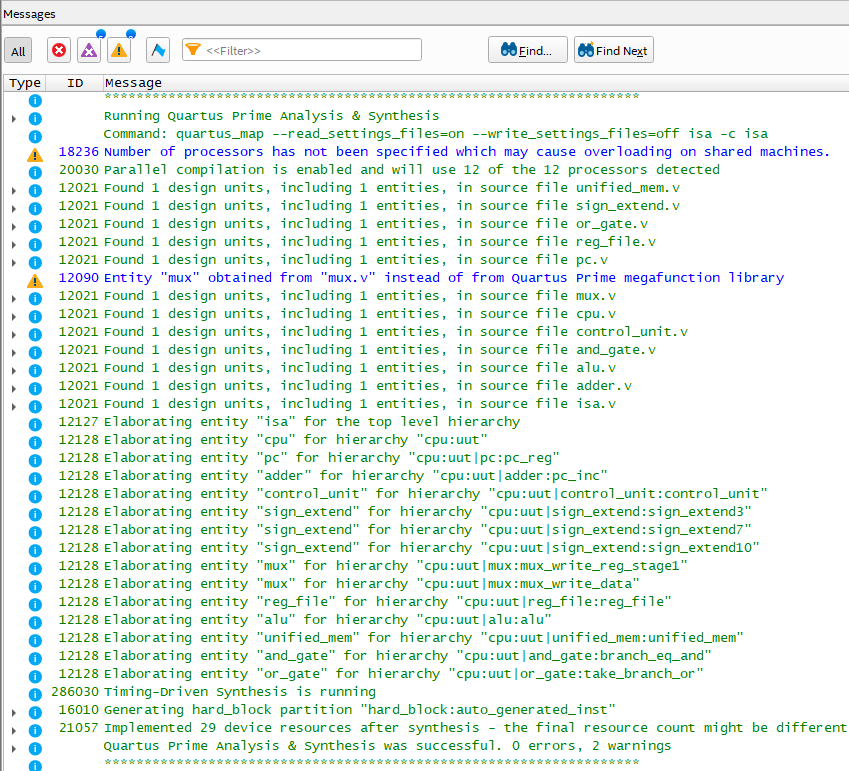
\includegraphics[width=1\linewidth]{transcript.png}
    \caption{Output Transcript}
\end{figure}

\begin{figure}
    \centering
    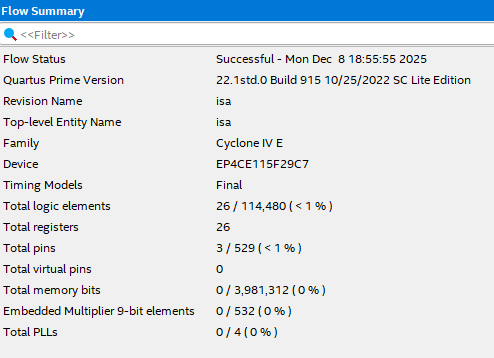
\includegraphics[width=0.75\linewidth]{flow_summary.png}
    \caption{Flow Summary}
\end{figure}

\section{Results}

\begin{figure}
    \centering
    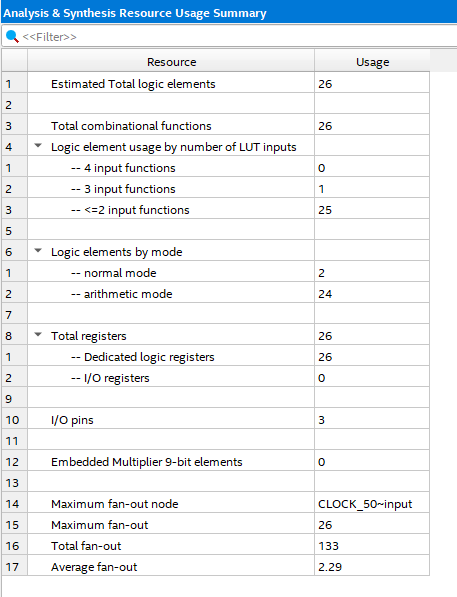
\includegraphics[width=0.75\linewidth]{resource_usage.png}
    \caption{Resource Usage}
\end{figure}

\begin{figure}
    \centering
    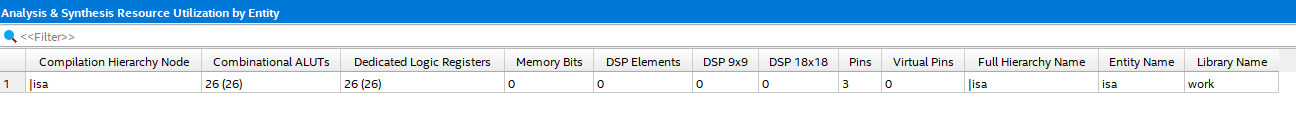
\includegraphics[width=1\linewidth]{resource_utilization.png}
    \caption{Resource Utilization}
\end{figure}

\begin{figure}
    \centering
    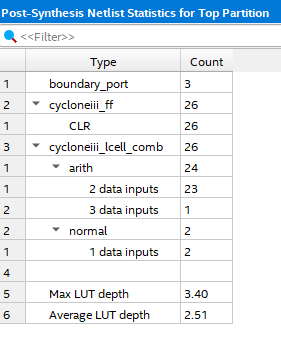
\includegraphics[width=0.5\linewidth]{netlist.png}
    \caption{Netlist Statistics}
\end{figure}

\begin{figure}
        \centering
        \includegraphics[width=0.75\linewidth]{de2-115.png}
        \caption{DE2-115 With LEDG8 Blinking}
        \label{fig:placeholder}
\end{figure}

Relative to the 32-bit, multi-module single-cycle MIPS processor studied in
class, this implementation is extremely lightweight:

\begin{itemize}
    \item The datapath is 16 bits wide instead of 32 bits.
    \item The register file contains 8 registers instead of 32.
    \item There is no pipelining, hazard detection, forwarding, or
          cache-like structures.
    \item The top-level design exposes only three I/O pins (clock,
          reset, and one LED), making integration minimal.
\end{itemize}

As a result, the logic utilization reported by Quartus (26 logic elements and
26 registers) is much smaller than the course MIPS design, which
typically consumes hundreds to several thousand logic elements and at least one
on-chip block RAM for instruction and data storage.

The measured utilization aligns appropriately with expectations:
the synthesized hardware contains only the clock divider and a small amount of
control and routing logic surrounding the CPU instance.vThere are no DSP blocks, block
RAMs, or PLLs inferred. The LUT depth and fanout statistics also reflect a
simple, shallow datapath with minimal combinational complexity.

Overall, the FPGA implementation confirms that the ISA design and CPU
architecture are compact and simpler than the
full-scale processor referred to in class, while still supporting all required
C-level constructs and program execution.

\appendix
\chapter{Full HDL Source Code}
This appendix provides the complete Verilog HDL implementation of the 16-bit processor, including the datapath, control unit, register file, ALU, unified memory, program counter, sign extension logic, and the full simulation
testbenches used for verification.

\section{Top-Level CPU Module}
\subsection*{cpu.v}
\begin{lstlisting}
module cpu (
    input  wire clk,
    input  wire reset
);
    // program counter and instruction fetch
    wire [15:0] pc;
    wire [15:0] pc_next;
    wire [15:0] instr;

    // pc register
    pc pc_reg(
        .clk(clk),
        .reset(reset),
        .pc_next(pc_next),
        .pc(pc)
    );

    // next pc logic
    wire [15:0] pc_plus_1;
    wire [15:0] branch_target;

    adder pc_inc(
        .in1(pc),
        .in2(16'h0001),
        .out(pc_plus_1)
    );

    // instruction decode
    wire [2:0] opcode = instr[15:13];
    wire [2:0] rs = instr[12:10];
    wire [2:0] rt = instr[9:7];
    wire [2:0] rd = instr[6:4];
    wire [2:0] funct = instr[3:1];
    wire iflag = instr[0];

    // immediates
    wire [2:0] imm3 = instr[9:7];  // shift, addi
    wire [6:0] imm7 = instr[6:0];  // branch, load/store offset
    wire [9:0] imm10 = instr[9:0];  // jump target, ldi

    // control unit
    wire [2:0] alu_op;
    wire [2:0] reg_dst;
    wire branch_eq, branch_ne;
    wire mem_read, mem_to_reg, mem_write;
    wire alu_src;
    wire reg_write;
    wire imm_to_reg, imm_jump, reg_jump;
    wire return_link;
    wire halt;

    control_unit control_unit(
        .opcode(opcode),
        .funct(funct),
        .alu_op(alu_op),
        .reg_dst(reg_dst),
        .branch_eq(branch_eq),
        .branch_ne(branch_ne),
        .mem_read(mem_read),
        .mem_to_reg(mem_to_reg),
        .mem_write(mem_write),
        .alu_src(alu_src),
        .reg_write(reg_write),
        .imm_to_reg(imm_to_reg),
        .imm_jump(imm_jump),
        .reg_jump(reg_jump),
	    .return_link(return_link),
	    .halt(halt)
    );

    // sign extension
    wire [15:0] imm3_ext;
    wire [15:0] imm7_ext;
    wire [15:0] imm10_ext;
   
    sign_extend #(.IN_WIDTH(3)) sign_extend3(
        .data_in(imm3),
        .data_extended(imm3_ext)
    );

    sign_extend #(.IN_WIDTH(7)) sign_extend7(
        .data_in(imm7),
        .data_extended(imm7_ext)
    );

    sign_extend #(.IN_WIDTH(10)) sign_extend10(
        .data_in(imm10),
        .data_extended(imm10_ext)
    );

    // register file
    wire [2:0] write_reg_stage1, write_reg_stage2, write_reg;
    wire [15:0] vrs;  // value of rs
    wire [15:0] vrt;  // value of rt (also used for stores)
    wire [15:0] wb_data, wb_data_med, wb_data_final; // write-back data to reg_file

    // select destination register: rd vs rt
    mux #(.WIDTH(3)) mux_write_reg_stage1(
        .in1(rt),
        .in2(rd),
        .select(reg_dst[0]),
        .out(write_reg_stage1)
    );

    // select destination register: vs I-type (rs)
    mux #(.WIDTH(3)) mux_write_reg_stage2(
        .in1(write_reg_stage1),
        .in2(rs),
        .select(reg_dst[1]),
        .out(write_reg_stage2)
    );

    // select destination register: jump link r7 = PC + 1
    mux #(.WIDTH(3)) mux_write_reg_final(
        .in1(write_reg_stage2),
        .in2(3'd7),
        .select(return_link),
        .out(write_reg)
    );

    mux mux_write_data(
        .in1(wb_data),
        .in2(imm10_ext),
        .select(imm_to_reg),
        .out(wb_data_med)
    );

    mux mux_write_data_final(
        .in1(wb_data_med),
        .in2(pc_plus_1),
        .select(return_link),
        .out(wb_data_final)
    );

    reg_file reg_file(
        .clk(clk),
        .enable(reg_write),
        .rs(rs),
        .rt(rt),
        .rd(write_reg),
        .wd(wb_data_final),
        .vrs(vrs),
        .vrt(vrt)
    );

    // arithmetic logic unit
    wire [15:0] alu_b;
    wire [15:0] alu_y;
    wire [15:0] alu_in2;  // value between muxes
    wire  alu_zero;

    // select small immediate based on iflag (vrt vs imm3_ext)
    mux mux_imm(
        .in1(vrt),
        .in2(imm3_ext),
        .select(iflag),
        .out(alu_in2)
    );

    // ALU second operand mux: alu_in2 vs imm7_ext
    mux mux_alu_src(
        .in1(alu_in2),
        .in2(imm7_ext),
        .select(alu_src),
        .out(alu_b)
    );

    alu alu(
        .a(vrs),
        .b(alu_b),
        .alu_op(alu_op),
        .y(alu_y),
        .zero(alu_zero)
    );

    // data memory
    wire [15:0] dmem_rdata;

    // unified memory (word-addressed)
    unified_mem unified_mem(
        .clk(clk),
        .i_addr(pc),
        .i_data(instr),
        .d_addr(alu_y), // address from ALU
        .d_wdata(vrt), // store data from rt
        .d_read(mem_read),
        .d_write(mem_write),
        .d_rdata(dmem_rdata)
    );

    // write-back mux (ALU result vs data memory)
    mux mux_writeback(
        .in1(alu_y),
        .in2(dmem_rdata),
        .select(mem_to_reg),
        .out(wb_data)
    );

    // branch_target = pc_plus_1 + imm7_ext
    adder branch_add(
        .in1(pc_plus_1),
        .in2(imm7_ext),
        .out(branch_target)
    );

    // branching and jumping
    wire take_beq, take_bne, take_branch;

    and_gate branch_eq_and(
        .in1(branch_eq),
        .in2(alu_zero),
        .out(take_beq)
    );

    and_gate branch_ne_and(
        .in1(branch_ne),
        .in2(!alu_zero),
        .out(take_bne)
    );

    or_gate take_branch_or(
        .in1(take_beq),
        .in2(take_bne),
        .out(take_branch)
    );

    // PC selection chain using muxes
    wire [15:0] pc_after_branch, pc_after_imm, pc_after_reg;

    // 1. branch vs fall-through
    mux mux_branch(
        .in1(pc_plus_1),
        .in2(branch_target),
        .select(take_branch),
        .out(pc_after_branch)
    );

    // 2. immediate jump vs previous
    mux mux_imm_jump(
        .in1(pc_after_branch),
        .in2(imm10_ext),  // jump_target_imm
        .select(imm_jump),
        .out(pc_after_imm)
    );

    // 3. register jump vs previous
    mux mux_reg_jump(
        .in1(pc_after_imm),
        .in2(vrs),  // jump_target_reg
        .select(reg_jump),
        .out(pc_after_reg)
    );

    // 4. pc halt
    mux mux_pc_select(
        .in1(pc_after_reg),
        .in2(pc),
        .select(halt),
        .out(pc_next)
    );

endmodule
\end{lstlisting}

\section{Control Unit}
\subsection*{control\_unit.v}
\begin{lstlisting}
`include "defs.vh"

module control_unit (
    input wire [2:0] opcode,
    input wire [2:0] funct,
    output reg [2:0] alu_op,
    output reg [2:0] reg_dst, // 00=rt, 01=rd, 10=rs
    output reg branch_eq,
    output reg branch_ne,
    output reg mem_read,
    output reg mem_to_reg,
    output reg mem_write,
    output reg alu_src,
    output reg reg_write,
    output reg imm_to_reg,
    output reg imm_jump,
    output reg reg_jump,
    output reg return_link,
    output reg halt
);
    
    // decode
    always @(*) begin
        alu_op = `ALU_NOP;
        reg_dst = 2'b00;  // default rt
        branch_eq = 0;
        branch_ne = 0;
        mem_read = 0;
        mem_to_reg = 0;
        mem_write = 0;
        alu_src = 0;
        reg_write = 0;
        imm_to_reg = 0;
        imm_jump = 0;
        reg_jump = 0;
	return_link = 0;
	halt = 0;
        case (opcode)
            `OP_R: begin
                reg_dst = 2'b01;  // write rd
                alu_src = 1'b0;  // use rt
                reg_write = 1'b1;
                case (funct)
                    `F_HALT: begin
                        reg_dst = 2'b00;
                        reg_write = 1'b0;
                        alu_op = `ALU_NOP;
                        halt = 1'b1;
                    end
                    `F_ADD: begin
                        alu_op = `ALU_ADD;
                    end
                    `F_SUB: begin
                        alu_op = `ALU_SUB;
                    end
                    `F_AND: begin
                        alu_op = `ALU_AND;
                    end
                    `F_OR: begin
                        alu_op = `ALU_OR;
                    end
                    `F_SLT: begin
                        alu_op = `ALU_SLT;
                    end
                    `F_SLL: begin
                        alu_op = `ALU_SLL;
                    end
                    `F_SRL: begin
                        alu_op = `ALU_SRL;
                    end
                    default: begin
                        alu_op = `ALU_NOP;
                    end
                endcase
            end
            `OP_ST: begin
                alu_op = `ALU_ADD;
                alu_src = 1'b1;  // use imm offset
                mem_write = 1'b1;
            end
            `OP_LD: begin
                alu_op = `ALU_ADD;
                alu_src = 1'b1;
                mem_read = 1'b1;
                mem_to_reg = 1'b1;  // writeback from mem
                reg_dst = 2'b00;  // write rt
                reg_write = 1'b1;
            end
            `OP_LDI: begin
                alu_op = `ALU_NOP;
                alu_src = 1'b1;
                reg_write = 1'b1;
                imm_to_reg = 1'b1;
		reg_dst = 2'b10;  // write rs
            end
            `OP_BEZ: begin
                alu_op = `ALU_SUB;
                branch_eq = 1'b1;
            end
            `OP_BNZ: begin
                alu_op = `ALU_SUB;
                branch_ne = 1'b1;
            end
            `OP_JL: begin
                imm_jump = 1'b1;
                reg_write = 1'b1;
                return_link = 1'b1;
            end
            `OP_JR: begin
                reg_jump = 1'b1;
            end
            default: begin
                halt = 1'b1;
                alu_op = `ALU_NOP;
            end
        endcase
    end

endmodule
\end{lstlisting}

\section{Datapath Components}

\subsection{ALU}
\subsubsection{alu.v}
\begin{lstlisting}
`include "defs.vh"

module alu (
    input wire [15:0] a, b,
    input wire [2:0] alu_op,
    output reg [15:0] y,
    output wire zero
);

    always @(*) begin
        case (alu_op)
            `ALU_ADD: y = a + b;
            `ALU_SUB: y = a - b;
            `ALU_AND: y = a & b;
            `ALU_OR: y = a | b;
            `ALU_SLT: y = ($signed(a) < $signed(b)) ? 16'h0001 : 16'h0000;
            `ALU_SLL: y = a << b[2:0];
            `ALU_SRL: y = a >> b[2:0];
            default: y = b;
        endcase
    end

    assign zero = (y == 16'h0000);
endmodule
\end{lstlisting}

\subsection{Register File}
\subsubsection{reg\_file.v}
\begin{lstlisting}
module reg_file (
    input wire clk,
    input wire enable,  // RegWrite enable
    input wire [2:0]  rs, rt, rd,  // input registers
    input wire [15:0] wd,  // write data
    output wire [15:0] vrs, vrt   // values read from registers
);
  
    reg [15:0] r[0:7];  // 8 x 16-bit registers

    // read registers
    assign vrs = (rs == 3'd0) ? 16'h0000 : r[rs];
    assign vrt = (rt == 3'd0) ? 16'h0000 : r[rt];

    // write on clock rising edge, ignore writes to r0
    always @(posedge clk) begin
        if (enable && (rd != 3'd0))
            r[rd] <= wd;
        r[0] <= 16'h0000; // keep $zero = 0
    end
endmodule
\end{lstlisting}

\subsection{Program Counter}
\subsubsection{pc.v}
\begin{lstlisting}
module pc (
    input wire clk,
    input wire reset,
    input wire [15:0] pc_next,  // what to load next
    output reg [15:0] pc  // current PC
);
    always @(posedge clk or posedge reset) begin
        if (reset)
            pc <= 16'h0000;
        else
            pc <= pc_next;
    end
endmodule
\end{lstlisting}

\subsection{Sign Extension Unit}
\subsubsection{sign\_extend.v}
\begin{lstlisting}
module sign_extend #(parameter IN_WIDTH = 7) (
    input [IN_WIDTH-1:0] data_in,
    output wire [15:0] data_extended
);

    // sign extend to 16 bits
    wire sign = data_in[IN_WIDTH-1];
    assign data_extended = {{(16-IN_WIDTH){sign}}, data_in};
    
endmodule
\end{lstlisting}

\subsection{Adder}
\subsubsection{adder.v}
\begin{lstlisting}
module adder (
    input [15:0] in1,
    input [15:0] in2,
    output wire [15:0] out
);

    assign out = in1 + in2;
    
endmodule
\end{lstlisting}

\subsection{MUX}
\subsubsection{mux.v}
\begin{lstlisting}
module mux #(parameter WIDTH = 16) (
    input wire [WIDTH-1:0] in1,
    input wire [WIDTH-1:0] in2,
    input wire select,
    output wire [WIDTH-1:0] out
);

assign out = select ? in2 : in1;
    
endmodule

\end{lstlisting}

\subsection{AND Gate}
\subsubsection{and\_gate.v}
\begin{lstlisting}
module and_gate (
    input in1,
    input in2,
    output wire out
);

    assign out = in1 & in2;
    
endmodule

\end{lstlisting}

\subsection{OR Gate}
\subsubsection{or\_gate.v}
\begin{lstlisting}
module or_gate (
    input in1,
    input in2,
    output wire out
);

    assign out = in1 | in2;
    
endmodule

\end{lstlisting}

\section{Unified Memory}

\subsection*{unified\_mem.v}
\begin{lstlisting}
module unified_mem (
    input clk,
    // instruction fetch (read-only)
    input wire [15:0] i_addr,
    output wire [15:0] i_data,
    // data access (load/store)
    input wire [15:0] d_addr,
    input wire [15:0] d_wdata,
    input wire d_read,
    input wire d_write,
    output wire [15:0] d_rdata
);

    reg [15:0] mem [0:1024-1];  // 1KiB memory space

    // instruction fetch
    assign i_data = mem[i_addr];
    // data read
    assign d_rdata = d_read ? mem[d_addr[8:0]] : 16'h0000;

    always @(posedge clk) begin
    // data write
        if (d_write)
            mem[d_addr] = d_wdata;
    end
    
endmodule
\end{lstlisting}

\section{Constant Definitions}
\subsection*{defs.vh}
\begin{lstlisting}
`ifndef DEFS_VH
`define DEFS_VH

// Opcodes
`define OP_R   3'b000
`define OP_ST  3'b001
`define OP_LD  3'b010
`define OP_LDI 3'b011
`define OP_BEZ 3'b100
`define OP_BNZ 3'b101
`define OP_JL  3'b110
`define OP_JR  3'b111

// Funct codes
`define F_ADD  3'b000
`define F_SUB  3'b001
`define F_AND  3'b010
`define F_OR   3'b011
`define F_SLT  3'b100
`define F_SLL  3'b101
`define F_SRL  3'b110
`define F_HALT 3'b111

// ALU opcodes
`define ALU_NOP 3'b000
`define ALU_ADD 3'b001
`define ALU_SUB 3'b010
`define ALU_AND 3'b011
`define ALU_OR  3'b100
`define ALU_SLT 3'b101
`define ALU_SLL 3'b110
`define ALU_SRL 3'b111

`endif // DEFS_VH
\end{lstlisting}

\section{Simulation Testbenches}

\subsection{Instructions Testbench}
\subsubsection{cpu\_tb.v}
\begin{lstlisting}
`timescale 1ns/1ps
`include "defs.vh"

module tb_cpu;

    reg clk;
    reg reset;

    // Unit under test
    cpu uut (
        .clk  (clk),
        .reset(reset)
    );

    // clock: 10ns period
    always #5 clk = ~clk;

    // ------------------------------
    // Encoding helpers (match ISA)
    // ------------------------------

    // R-Type:
    // [15:13] op
    // [12:10] rs
    // [ 9:7 ] rt_or_imm
    // [ 6:4 ] rd
    // [ 3:1 ] funct
    // [ 0   ] iflag
    function [15:0] enc_rtype;
        input [2:0] op;
        input [2:0] rs;
        input [2:0] rt_or_imm;
        input [2:0] rd;
        input [2:0] funct;
        input       iflag;
        begin
            enc_rtype = {op, rs, rt_or_imm, rd, funct, iflag};
        end
    endfunction

    // LS-Type:
    // [15:13] op
    // [12:10] rs   (base)
    // [ 9:7 ] rt   (reg)
    // [ 6:0 ] imm7 (offset)
    function [15:0] enc_ls;
        input [2:0] op;
        input [2:0] rs;
        input [2:0] rt;
        input [6:0] imm7;
        begin
            enc_ls = {op, rs, rt, imm7};
        end
    endfunction

    // IJ-Type:
    // [15:13] op
    // [12:10] rd_or_rs
    // [ 9:0 ] imm10
    function [15:0] enc_ij;
        input [2:0] op;
        input [2:0] rd;
        input [9:0] imm10;
        begin
            enc_ij = {op, rd, imm10};
        end
    endfunction

    integer i;

    initial begin
        clk   = 1'b1;
        reset = 1'b1;

        // Clear instruction & data memory
        for (i = 0; i < 64; i = i + 1) begin
            uut.unified_mem.mem[i] = 16'h0000;
        end

        // Clear registers (r[])
        for (i = 0; i < 8; i = i + 1) begin
            uut.reg_file.r[i] = 16'h0000;
        end

        // ----------------------------------------------------
        // Program to exercise all instructions
        // ----------------------------------------------------
        //  0: LDI r1, 10
        uut.unified_mem.mem[0]  = enc_ij(`OP_LDI, 3'd1, 10'd10);

        //  1: LDI r2, 3
        uut.unified_mem.mem[1]  = enc_ij(`OP_LDI, 3'd2, 10'd3);

        //  2: ADD  r3 = r1 + r2    (10 + 3 = 13)
        uut.unified_mem.mem[2]  = enc_rtype(`OP_R, 3'd1, 3'd2, 3'd3, `F_ADD, 1'b0);

        //  3: SUB  r4 = r1 - r2    (10 - 3 = 7)
        uut.unified_mem.mem[3]  = enc_rtype(`OP_R, 3'd1, 3'd2, 3'd4, `F_SUB, 1'b0);

        //  4: AND  r5 = r1 & r2    (10 & 3 = 2)
        uut.unified_mem.mem[4]  = enc_rtype(`OP_R, 3'd1, 3'd2, 3'd5, `F_AND, 1'b0);

        //  5: OR   r6 = r1 | r2    (10 | 3 = 11)
        uut.unified_mem.mem[5]  = enc_rtype(`OP_R, 3'd1, 3'd2, 3'd6, `F_OR, 1'b0);

        //  6: SLT  r7 = (r2 < r1) ? 1 : 0   (3 < 10 --> 1)
        uut.unified_mem.mem[6]  = enc_rtype(`OP_R, 3'd2, 3'd1, 3'd7, `F_SLT, 1'b0);

        //  7: ADDI r1 = r1 + 1     (iflag=1, imm3=1)
        uut.unified_mem.mem[7]  = enc_rtype(`OP_R, 3'd1, 3'd1, 3'd1, `F_ADD, 1'b1);

        //  8: SLL  r2 << 1         (3 << 1 = 6)
        uut.unified_mem.mem[8]  = enc_rtype(`OP_R, 3'd2, 3'd1, 3'd2, `F_SLL, 1'b1);

        //  9: SRL  r2 >> 1         (6 >> 1 = 3)
        uut.unified_mem.mem[9]  = enc_rtype(`OP_R, 3'd2, 3'd1, 3'd2, `F_SRL, 1'b1);

        // 10: ST   M[r0 + 31] <- r3 (addr = 31)
        uut.unified_mem.mem[10] = enc_ls(`OP_ST, 3'd0, 3'd3, 7'd31);

        // 11: LD   r4 <- M[r0 + 31] (=> 13)
        uut.unified_mem.mem[11] = enc_ls(`OP_LD, 3'd0, 3'd4, 7'd31);

        // 12: BEZ  r4, +1          (r4 != 0 so NOT taken; executes at 13)
        uut.unified_mem.mem[12] = enc_ij(`OP_BEZ, 3'd4, 10'd1);

        // 13: BNZ  r4, +1          (r4 != 0 so taken; skips 14)
        uut.unified_mem.mem[13] = enc_ij(`OP_BNZ, 3'd4, 10'd1);

        // 14: LDI  r5, 99          (should be skipped if BNZ works)
        uut.unified_mem.mem[14] = enc_ij(`OP_LDI, 3'd5, 10'd99);

        // 15: JL   18          (jump to PC = 18, link in r7)
        uut.unified_mem.mem[15] = enc_ij(`OP_JL, 3'd7, 10'd18);

        // 16: HALT (END)
        uut.unified_mem.mem[16] = enc_rtype(`OP_R, 3'd0, 3'd0, 3'd0, `F_HALT, 1'b0);

        // 17: NOP (0)
        uut.unified_mem.mem[17] = 16'h0000;

        // 18: LDI  r1, 42          (function body)
        uut.unified_mem.mem[18] = enc_ij(`OP_LDI, 3'd1, 10'd42);

        // 19: JR   r7              (return to whatever JL stored)
        uut.unified_mem.mem[19] = enc_ij(`OP_JR, 3'd7, 10'd0);

        // 20: ADDI r1 = r1 + 1     (should not execute after JR if link worked)
        uut.unified_mem.mem[20] = enc_rtype(`OP_R, 3'd1, 3'd1, 3'd1, `F_ADD, 1'b1);
        
	// Release reset after 20 time units (~2 cycles)
        #20;
        reset = 1'b0;

        // Run long enough to step through everything
        #190;

        reset = 1'b1;
	#20;
        reset = 1'b0;
	#20;

        $display("\n==== FINAL STATE ====");
        for (i = 0; i < 8; i = i + 1) begin
            $display("R%0d = 0x%04h (%0d)", i, uut.reg_file.r[i], uut.reg_file.r[i]);
        end

        $display("MEM[0..31]:");
        for (i = 0; i < 32; i = i + 1) begin
            $display("MEM[%0d] = 0x%04h (%0d)", i, uut.unified_mem.mem[i], uut.unified_mem.mem[i]);
        end

        $finish;
    end

    // ----------------------------------------------------
    // Cycle-by-cycle debug print with instruction labels
    // ----------------------------------------------------
    always @(posedge clk) begin
        if (reset) begin
            $display("----- t=%0t (RESET ACTIVE) -----", $time);
            $display("PC = %0d", uut.pc);
            $display("-----------------------------\n");
        end else begin
            $display("----- t=%0t -----", $time);
            $display("PC     = %0d", uut.pc);
            $display("INSTR  = 0x%04h", uut.instr);
            $display("DECODE : opcode=%b rs=%0d rt=%0d rd=%0d funct=%b iflag=%b",
                     uut.instr[15:13], uut.instr[12:10],
                     uut.instr[9:7],   uut.instr[6:4],
                     uut.instr[3:1],   uut.instr[0]);

            // Label the current instruction and its intended RTL
            case (uut.pc)
                0: begin
                    $display("INST   : [PC 0] LDI r1, 10");
                    $display("RTL    : r1 = 10");
                end
                1: begin
                    $display("INST   : [PC 1] LDI r2, 3");
                    $display("RTL    : r2 = 3");
                end
                2: begin
                    $display("INST   : [PC 2] ADD r3, r1, r2");
                    $display("RTL    : r3 = r1 + r2 = 10 + 3 = 13");
                end
                3: begin
                    $display("INST   : [PC 3] SUB r4, r1, r2");
                    $display("RTL    : r4 = r1 - r2 = 10 - 3 = 7 (later overwritten by LD)");
                end
                4: begin
                    $display("INST   : [PC 4] AND r5, r1, r2");
                    $display("RTL    : r5 = r1 & r2 = 10 & 3 = 2");
                end
                5: begin
                    $display("INST   : [PC 5] OR r6, r1, r2");
                    $display("RTL    : r6 = r1 | r2 = 10 | 3 = 11");
                end
                6: begin
                    $display("INST   : [PC 6] SLT r7, r2, r1");
                    $display("RTL    : r7 = (r2 < r1) ? 1 : 0 = (3 < 10) ? 1 : 0 = 1");
                end
                7: begin
                    $display("INST   : [PC 7] ADDI r1, r1, +1");
                    $display("RTL    : r1 = r1 + 1  (11 after this if it was 10)");
                end
                8: begin
                    $display("INST   : [PC 8] SLL r2, r2, 1");
                    $display("RTL    : r2 = r2 << 1  (3 << 1 = 6)");
                end
                9: begin
                    $display("INST   : [PC 9] SRL r2, r2, 1");
                    $display("RTL    : r2 = r2 >> 1  (6 >> 1 = 3)");
                end
                10: begin
                    $display("INST   : [PC 10] ST [r0 + 31] <- r3");
                    $display("RTL    : MEM[31] = r3 = 13");
                end
                11: begin
                    $display("INST   : [PC 11] LD r4 <- [r0 + 31]");
                    $display("RTL    : r4 = MEM[31] = 13");
                end
                12: begin
                    $display("INST   : [PC 12] BEZ r4, +1");
                    $display("RTL    : if (r4 == 0) PC += offset; here r4 != 0 so NOT taken");
                end
                13: begin
                    $display("INST   : [PC 13] BNZ r4, +1");
                    $display("RTL    : if (r4 != 0) PC += offset; here r4 != 0 so TAKEN (skip PC 14)");
                end
                14: begin
                    $display("INST   : [PC 14] LDI r5, 99");
                    $display("RTL    : r5 = 99 (should be skipped if BNZ at PC 13 worked)");
                end
                15: begin
                    $display("INST   : [PC 15] JL 18");
                    $display("RTL    : r7 = return_addr; PC jumps to 18");
                end
                16: begin
                    $display("INST   : [PC 16] HALT (end of program)");
                    $display("RTL    : Stop execution");
                end
                17: begin
                    $display("INST   : [PC 17] NOP (0)");
                    $display("RTL    : No operation");
                end
                18: begin
                    $display("INST   : [PC 18] LDI r1, 42");
                    $display("RTL    : r1 = 42 (function body after JL)");
                end
                19: begin
                    $display("INST   : [PC 19] JR r7");
                    $display("RTL    : PC = r7 (return to caller)");
                end
                20: begin
                    $display("INST   : [PC 20] ADDI r1, r1, +1");
                    $display("RTL    : r1 = r1 + 1  (42 + 1 = 43 not executed if JR returned correctly)");
                end
                default: begin
                    $display("INST   : [PC %0d] (no label defined)", uut.pc);
                end
            endcase

            // Normal signal trace
            $display("CONTROL: alu_op=%b reg_dst=%b reg_write=%b mem_read=%b mem_write=%b branch_ez=%b branch_nz=%b imm_jump=%b reg_jump=%b return_link=%b halt=%b",
                     uut.alu_op, uut.reg_dst, uut.alu_src,
                     uut.mem_to_reg, uut.reg_write,
                     uut.mem_read, uut.mem_write,
                     uut.branch_eq, uut.branch_ne, uut.imm_jump, uut.reg_jump, uut.return_link, uut.halt);

            $display("ALU    : vrs(a)=%0d  alu_b(b)=%0d  -> y=%0d  zero=%b",
                     uut.vrs, uut.alu_b, uut.alu_y, uut.alu_zero);

            $display("WB     : write_reg=%0d  wb_data=%0d  reg_write=%b",
                     uut.write_reg, uut.wb_data, uut.reg_write);

            $display("REGS   : r0=%0d r1=%0d r2=%0d r3=%0d r4=%0d r5=%0d r6=%0d r7=%0d",
                     uut.reg_file.r[0], uut.reg_file.r[1], uut.reg_file.r[2], uut.reg_file.r[3],
                     uut.reg_file.r[4], uut.reg_file.r[5], uut.reg_file.r[6], uut.reg_file.r[7]);

            $display("MEM    : M[31]=%0d M[30]=%0d M[1]=%0d M[0]=%0d",
                     uut.unified_mem.mem[31], uut.unified_mem.mem[30],
                     uut.unified_mem.mem[1], uut.unified_mem.mem[0]);
            $display("-----------------------------\n");
        end
    end

endmodule
\end{lstlisting}

\subsection{Control Flow Testbench}
\subsubsection{cpu\_flow\_tb.v}
\begin{lstlisting}
`timescale 1ns/1ps
`include "defs.vh"

module tb_cpu_flow;

    reg clk;
    reg reset;

    // Unit under test
    cpu uut (
        .clk  (clk),
        .reset(reset)
    );

    // clock: 10ns period
    always #5 clk = ~clk;

    // ------------------------------
    // Encoding helpers (match ISA)
    // ------------------------------

    // R-Type:
    // [15:13] op
    // [12:10] rs
    // [ 9:7 ] rt_or_imm
    // [ 6:4 ] rd
    // [ 3:1 ] funct
    // [ 0   ] iflag
    function [15:0] enc_rtype;
        input [2:0] op;
        input [2:0] rs;
        input [2:0] rt_or_imm;
        input [2:0] rd;
        input [2:0] funct;
        input       iflag;
        begin
            enc_rtype = {op, rs, rt_or_imm, rd, funct, iflag};
        end
    endfunction

    // LS-Type:
    // [15:13] op
    // [12:10] rs   (base)
    // [ 9:7 ] rt   (reg)
    // [ 6:0 ] imm7 (offset)
    function [15:0] enc_ls;
        input [2:0] op;
        input [2:0] rs;
        input [2:0] rt;
        input [6:0] imm7;
        begin
            enc_ls = {op, rs, rt, imm7};
        end
    endfunction

    // IJ-Type:
    // [15:13] op
    // [12:10] rd_or_rs
    // [ 9:0 ] imm10
    function [15:0] enc_ij;
        input [2:0] op;
        input [2:0] rd;
        input [9:0] imm10;
        begin
            enc_ij = {op, rd, imm10};
        end
    endfunction

    integer i;

    initial begin
        clk   = 1'b0;
        reset = 1'b1;

        // ----------------------------------------------------
        // Unified memory:
        //   - Low addresses (e.g., 0..63) used for instructions
        //   - Higher addresses reserved for data
        // ----------------------------------------------------
        for (i = 0; i < 64; i = i + 1) begin
            uut.unified_mem.mem[i] = 16'h0000;
        end

        // Clear registers (r[])
        for (i = 0; i < 8; i = i + 1) begin
            uut.reg_file.r[i] = 16'h0000;
        end

        // ----------------------------------------------------
        // Program to exercise control structures:
        //   - if / else
        //   - while loop
        //   - for loop
        //   - function call / return (JL / JR)
        //
        // Registers used:
        //   r1, r2 : values / bounds (a, b, etc.)
        //   r3     : if-else result (c)
        //   r4     : accumulator (sum)
        //   r5     : while-loop index i
        //   r6     : for-loop index j
        //   r7     : link register ($ra) and branch temp
        // ----------------------------------------------------

        // ---------------------------------------------
        // C: int a = 2, b = 3;
        // ---------------------------------------------
        //  0: LDI r1, 2   ; a = 2
        uut.unified_mem.mem[0]  = enc_ij(`OP_LDI, 3'd1, 10'd2);
        //  1: LDI r2, 3   ; b = 3
        uut.unified_mem.mem[1]  = enc_ij(`OP_LDI, 3'd2, 10'd3);

        // ---------------------------------------------
        // C: if (a < b) { c = 1; } else { c = 2; }
        //    a in r1, b in r2, c in r3
        // ---------------------------------------------
        //  2: SLT r4, r1, r2    ; r4 = (a < b)
        uut.unified_mem.mem[2]  = enc_rtype(`OP_R, 3'd1, 3'd2, 3'd4, `F_SLT, 1'b0);
        //  3: BEZ r4, +2        ; if !cond -> jump to else at PC = 6
        //      PC_target = 3 + 1 + 2 = 6
        uut.unified_mem.mem[3]  = enc_ij(`OP_BEZ, 3'd4, 10'd2);
        //  4: LDI r3, 1         ; then: c = 1
        uut.unified_mem.mem[4]  = enc_ij(`OP_LDI, 3'd3, 10'd1);
        //  5: BNZ r4, +1        ; jump to after_if at PC = 7
        //      PC_target = 5 + 1 + 1 = 7
        uut.unified_mem.mem[5]  = enc_ij(`OP_BNZ, 3'd4, 10'd1);
        //  6: LDI r3, 2         ; else: c = 2
        uut.unified_mem.mem[6]  = enc_ij(`OP_LDI, 3'd3, 10'd2);
        //  7: after_if:

        // ---------------------------------------------
        // C: while (i < 2) { i++; }
        //    i in r5, bound 2 in r1
        // ---------------------------------------------
        //  7: LDI r5, 0         ; i = 0
        uut.unified_mem.mem[7]  = enc_ij(`OP_LDI, 3'd5, 10'd0);
        //  8: loop_top: SLT r6, r5, r1  ; r6 = (i < 3)
        uut.unified_mem.mem[8]  = enc_rtype(`OP_R, 3'd5, 3'd1, 3'd6, `F_SLT, 1'b0);
        //  9: BEZ r6, +2        ; if !(i < 3) -> loop_end at PC = 12
        //      PC_target = 9 + 1 + 2 = 12
        uut.unified_mem.mem[9]  = enc_ij(`OP_BEZ, 3'd6, 10'd2);
        // 10: ADDI r5, r5, +1   ; i++
        //      rs = 5, imm3 = 1, rd = 5
        uut.unified_mem.mem[10] = enc_rtype(`OP_R, 3'd5, 3'd1, 3'd5, `F_ADD, 1'b1);
        // 11: BNZ r6, -4        ; back to loop_top (PC = 8)
        //      offset = 8 - (11 + 1) = -4 -> 10-bit two's-comp = 1020
        uut.unified_mem.mem[11] = enc_ij(`OP_BNZ, 3'd6, 10'd1020);
        // 12: loop_end:

        // ---------------------------------------------
        // C: for (j = 0; j < b; j++) { sum += j; }
        //    j in r6, sum in r4, b in r2 (=3)
        // ---------------------------------------------
        // 12: LDI r6, 0         ; j = 0
        uut.unified_mem.mem[12] = enc_ij(`OP_LDI, 3'd6, 10'd0);
        // 13: LDI r4, 0         ; sum = 0
        uut.unified_mem.mem[13] = enc_ij(`OP_LDI, 3'd4, 10'd0);
        // 14: for_top: SLT r7, r6, r2  ; r7 = (j < b)
        uut.unified_mem.mem[14] = enc_rtype(`OP_R, 3'd6, 3'd2, 3'd7, `F_SLT, 1'b0);
        // 15: BEZ r7, +3        ; if !(j < b) -> for_end at PC = 19
        //      PC_target = 15 + 1 + 3 = 19
        uut.unified_mem.mem[15] = enc_ij(`OP_BEZ, 3'd7, 10'd3);
        // 16: ADD r4, r4, r6    ; sum += j
        uut.unified_mem.mem[16] = enc_rtype(`OP_R, 3'd4, 3'd6, 3'd4, `F_ADD, 1'b0);
        // 17: ADDI r6, r6, +1   ; j++
        uut.unified_mem.mem[17] = enc_rtype(`OP_R, 3'd6, 3'd1, 3'd6, `F_ADD, 1'b1);
        // 18: BNZ r7, -5        ; back to for_top (PC = 14)
        //      offset = 14 - (18 + 1) = -5 -> 10-bit two's-comp = 1019
        uut.unified_mem.mem[18] = enc_ij(`OP_BNZ, 3'd7, 10'd1019);
        // 19: for_end:

        // ---------------------------------------------
        // C: int inc(int x) { return x + 1; }
        //    r1 = inc(10);
        //    x in r1, return in r1, r7 as $ra
        // ---------------------------------------------
        // 20: LDI r1, 10        ; argument x = 10
        uut.unified_mem.mem[20] = enc_ij(`OP_LDI, 3'd1, 10'd10);
        // 21: JL 24             ; call inc at PC = 24, link in r7
        uut.unified_mem.mem[21] = enc_ij(`OP_JL, 3'd7, 10'd24);
        // 22: ADDI r1, r1, 0    ; no-op, should see r1 = 11 if call/ret worked
        //      rs = 1, imm3 = 0, rd = 1
        uut.unified_mem.mem[22] = enc_rtype(`OP_R, 3'd1, 3'd0, 3'd1, `F_ADD, 1'b1);
        // 23: HALT              ; end of main program
        uut.unified_mem.mem[23] = enc_rtype(`OP_R, 3'd0, 3'd0, 3'd0, `F_HALT, 1'b0);

        // Function inc: int inc(int x) { return x + 1; }
        // 24: ADDI r1, r1, +1   ; r1 = r1 + 1
        uut.unified_mem.mem[24] = enc_rtype(`OP_R, 3'd1, 3'd1, 3'd1, `F_ADD, 1'b1);
        // 25: JR r7             ; return to caller
        uut.unified_mem.mem[25] = enc_ij(`OP_JR, 3'd7, 10'd0);

        // Release reset after 20 time units (~2 cycles)
        #20;
        reset = 1'b0;

        // Run long enough to step through everything (loops + call)
        #430;

        $display("\n==== FINAL STATE ====");
        for (i = 0; i < 8; i = i + 1) begin
            $display("R%0d = 0x%04h (%0d)", i, uut.reg_file.r[i], uut.reg_file.r[i]);
        end

        // Show a slice of unified memory:
        $display("MEM[0..31]:");
        for (i = 0; i < 32; i = i + 1) begin
            $display("MEM[%0d] = 0x%04h (%0d)", i, uut.unified_mem.mem[i], uut.unified_mem.mem[i]);
        end

        $finish;
    end

    // ----------------------------------------------------
    // Cycle-by-cycle debug print with instruction labels
    // ----------------------------------------------------
    always @(negedge clk) begin
        if (reset) begin
            $display("----- t=%0t (RESET ACTIVE) -----", $time);
            $display("PC = %0d", uut.pc);
            $display("-----------------------------\n");
        end else begin
            $display("----- t=%0t -----", $time);
            $display("PC     = %0d", uut.pc);
            $display("INSTR  = 0x%04h", uut.instr);
            $display("DECODE : opcode=%b rs=%0d rt=%0d rd=%0d funct=%b iflag=%b",
                     uut.instr[15:13], uut.instr[12:10],
                     uut.instr[9:7],   uut.instr[6:4],
                     uut.instr[3:1],   uut.instr[0]);

            // Label the current instruction and its intended C/RTL meaning
            case (uut.pc)
                0: begin
                    $display("INST   : [PC 0] LDI r1, 2");
                    $display("C      : int a = 2;");
                end
                1: begin
                    $display("INST   : [PC 1] LDI r2, 3");
                    $display("C      : int b = 3;");
                end
                2: begin
                    $display("INST   : [PC 2] SLT r4, r1, r2");
                    $display("C      : cond = (a < b);");
                    $display("RTL    : r4 = (r1 < r2) ? 1 : 0;");
                end
                3: begin
                    $display("INST   : [PC 3] BEZ r4, +2");
                    $display("C      : if (!cond) goto else;");
                end
                4: begin
                    $display("INST   : [PC 4] LDI r3, 1");
                    $display("C      : then: c = 1;");
                end
                5: begin
                    $display("INST   : [PC 5] BNZ r4, +1");
                    $display("C      : goto after_if;");
                end
                6: begin
                    $display("INST   : [PC 6] LDI r3, 2");
                    $display("C      : else: c = 2;");
                end
                7: begin
                    $display("INST   : [PC 7] LDI r5, 0");
                    $display("C      : int i = 0;  // while-loop init");
                end
                8: begin
                    $display("INST   : [PC 8] SLT r6, r5, r1");
                    $display("C      : while (i < 2) {");
                    $display("RTL    : r6 = (r5 < r1) ? 1 : 0;");
                end
                9: begin
                    $display("INST   : [PC 9] BEZ r6, +2");
                    $display("C      : if (!(i < 2)) break;");
                end
                10: begin
                    $display("INST   : [PC 10] ADDI r5, r5, +1");
                    $display("C      : i++;");
                end
                11: begin
                    $display("INST   : [PC 11] BNZ r6, -4");
                    $display("C      : loop back to while condition;");
                end
                12: begin
                    $display("INST   : [PC 12] LDI r6, 0");
                    $display("C      : int j = 0;  // for-loop init");
                end
                13: begin
                    $display("INST   : [PC 13] LDI r4, 0");
                    $display("C      : int sum = 0;");
                end
                14: begin
                    $display("INST   : [PC 14] SLT r7, r6, r2");
                    $display("C      : for (j < 3) {");
                    $display("RTL    : r7 = (r6 < r2) ? 1 : 0;");
                end
                15: begin
                    $display("INST   : [PC 15] BEZ r7, +3");
                    $display("C      : if (!(j < b)) break;");
                end
                16: begin
                    $display("INST   : [PC 16] ADD r4, r4, r6");
                    $display("C      : sum += j;");
                end
                17: begin
                    $display("INST   : [PC 17] ADDI r6, r6, +1");
                    $display("C      : j++;");
                end
                18: begin
                    $display("INST   : [PC 18] BNZ r7, -5");
                    $display("C      : loop back to for condition;");
                end
                19: begin
                    $display("INST   : [PC 19] NOP (for_end)");
                    $display("C      : end of for-loop;");
                end
                20: begin
                    $display("INST   : [PC 20] LDI r1, 10");
                    $display("C      : r1 = 10;  // argument x for inc(x)");
                end
                21: begin
                    $display("INST   : [PC 21] JL 24");
                    $display("C      : call inc;");
                    $display("RTL    : r7 = return_addr; PC = 24;");
                end
                22: begin
                    $display("INST   : [PC 22] ADDI r1, r1, 0");
                    $display("C      : // after return, r1 should be x+1 = 11;");
                end
                23: begin
                    $display("INST   : [PC 23] HALT");
                    $display("C      : end of main;");
                end
                24: begin
                    $display("INST   : [PC 24] ADDI r1, r1, +1");
                    $display("C      : int inc(int x) { return x + 1; }");
                end
                25: begin
                    $display("INST   : [PC 25] JR r7");
                    $display("C      : return from inc;");
                end
                default: begin
                    $display("INST   : [PC %0d] (no label defined)", uut.pc);
                end
            endcase

            // Normal signal trace
            $display("CONTROL: alu_op=%b reg_dst=%b alu_src=%b mem_to_reg=%b reg_write=%b mem_read=%b mem_write=%b branch_ez=%b branch_nz=%b imm_jump=%b reg_jump=%b return_link=%b halt=%b",
                     uut.alu_op, uut.reg_dst, uut.alu_src,
                     uut.mem_to_reg, uut.reg_write,
                     uut.mem_read, uut.mem_write,
                     uut.branch_eq, uut.branch_ne, uut.imm_jump, uut.reg_jump, uut.return_link, uut.halt);

            $display("ALU    : vrs(a)=%0d  alu_b(b)=%0d  -> y=%0d  zero=%b",
                     uut.vrs, uut.alu_b, uut.alu_y, uut.alu_zero);

            $display("WB     : write_reg=%0d  wb_data=%0d  reg_write=%b",
                     uut.write_reg, uut.wb_data, uut.reg_write);

            $display("REGS   : r0=%0d r1=%0d r2=%0d r3=%0d r4=%0d r5=%0d r6=%0d r7=%0d",
                     uut.reg_file.r[0], uut.reg_file.r[1], uut.reg_file.r[2], uut.reg_file.r[3],
                     uut.reg_file.r[4], uut.reg_file.r[5], uut.reg_file.r[6], uut.reg_file.r[7]);

            $display("MEM    : M[0]=%0d M[1]=%0d M[2]=%0d M[3]=%0d",
                     uut.unified_mem.mem[0], uut.unified_mem.mem[1],
                     uut.unified_mem.mem[2], uut.unified_mem.mem[3]);
            $display("-----------------------------\n");
        end
    end

endmodule

\end{lstlisting}

\section{Top-Level Hardware Integration Module}
\subsection*{isa.v}
\label{appendix:hardwaremodule}
\begin{lstlisting}
/*
PIN ASSIGNMENTS:
set_location_assignment PIN_Y2  -to CLOCK_50
set_location_assignment PIN_M23 -to KEY0
set_location_assignment PIN_F17 -to LEDG8
*/
module isa (
    input wire CLOCK_50,
    input wire KEY0,
    output reg LEDG8
);

	wire reset = ~KEY0;
	reg clk;
	reg [25:0] counter;
	
	always @(posedge CLOCK_50 or posedge reset) begin
		if(reset)
			counter <= 26'd0;
		else
			counter <= counter + 26'd1;
	end
	
	always @(*) begin
		LEDG8 <= counter[25];  // blink for clock
		clk <= counter[25];
	end
	
	cpu uut (
		.clk(clk),
		.reset(reset)
	);
endmodule
\end{lstlisting}

\end{document}
